% =============================================================================
% Hexplain — Rapport de Stage — main.tex
% Compilé avec pdflatex + biber sur Overleaf
% =============================================================================

\documentclass[12pt, a4paper, twoside]{report}

% =============================================================================
% Hexplain — Rapport de Stage
% Préambule LaTeX — packages, configurations, commandes personnalisées
% Compatible Overleaf (pdflatex)
% =============================================================================

% --- Encodage & langue ---
\usepackage[utf8]{inputenc}
\usepackage[T1]{fontenc}
\usepackage[french]{babel}
\usepackage{csquotes}

% --- Mise en page ---
\usepackage[a4paper, top=2.5cm, bottom=2.5cm, left=3cm, right=2.5cm]{geometry}
\usepackage{setspace}
\onehalfspacing
\usepackage{emptypage}    % Supprime en-têtes/pieds sur pages vides

% --- Typographie ---
\usepackage{lmodern}
\usepackage{microtype}

% --- En-têtes et pieds de page ---
\usepackage{fancyhdr}
\pagestyle{fancy}
\fancyhf{}
\fancyhead[L]{\small\textit{Hexplain — Pipeline d'analyse statique de binaires PE/ELF intégrant des LLM}}
\fancyhead[R]{\small\textit{AIT OIHMANE Lahsen}}
\fancyfoot[C]{\thepage}
\renewcommand{\headrulewidth}{0.4pt}
\renewcommand{\footrulewidth}{0pt}

% --- Style de page pour les débuts de chapitre ---
\fancypagestyle{plain}{%
  \fancyhf{}
  \fancyfoot[C]{\thepage}
  \renewcommand{\headrulewidth}{0pt}
}

% --- Couleurs ---
\usepackage[dvipsnames,svgnames,table]{xcolor}
\definecolor{indigodark}{RGB}{55,48,163}
\definecolor{indigo}{RGB}{79,70,229}
\definecolor{indigolight}{RGB}{165,180,252}
\definecolor{slategray}{RGB}{71,85,105}
\definecolor{slatelight}{RGB}{248,250,252}
\definecolor{codebackground}{RGB}{248,249,250}
\definecolor{framegray}{RGB}{209,213,219}
\definecolor{warnorange}{RGB}{217,119,6}
\definecolor{successgreen}{RGB}{5,150,105}
\definecolor{dangerred}{RGB}{185,28,28}

% --- Graphiques & images ---
\usepackage{graphicx}
\graphicspath{{img/}}
\usepackage{float}
\usepackage{caption}
\usepackage{subcaption}
\captionsetup{
  font=small,
  labelfont=bf,
  labelsep=period,
  justification=centering,
  skip=6pt
}

% --- Tableaux ---
\usepackage{booktabs}
\usepackage{tabularx}
\usepackage{longtable}
\usepackage{multirow}
\usepackage{array}
\usepackage{makecell}
\renewcommand{\arraystretch}{1.3}

% --- Listes ---
\usepackage{enumitem}
\setlist[itemize]{leftmargin=*, topsep=4pt, itemsep=2pt}
\setlist[enumerate]{leftmargin=*, topsep=4pt, itemsep=2pt}

% --- Code source ---
\usepackage{listings}
\lstdefinestyle{hexplainstyle}{
  backgroundcolor=\color{codebackground},
  basicstyle=\ttfamily\footnotesize,
  breakatwhitespace=false,
  breaklines=true,
  captionpos=b,
  commentstyle=\color{slategray}\itshape,
  frame=single,
  rulecolor=\color{framegray},
  keywordstyle=\color{indigo}\bfseries,
  numberstyle=\tiny\color{slategray},
  numbers=left,
  numbersep=8pt,
  showspaces=false,
  showstringspaces=false,
  showtabs=false,
  stringstyle=\color{successgreen},
  tabsize=2,
  xleftmargin=12pt,
  xrightmargin=4pt,
  aboveskip=8pt,
  belowskip=8pt
}
\lstset{style=hexplainstyle}

% --- Boîtes colorées ---
\usepackage{tcolorbox}
\tcbuselibrary{most}

\newtcolorbox{notebox}{
  colback=slatelight,
  colframe=indigodark,
  fonttitle=\bfseries,
  title=Note,
  left=6pt, right=6pt, top=4pt, bottom=4pt
}

\newtcolorbox{warnbox}{
  colback=yellow!10,
  colframe=warnorange,
  fonttitle=\bfseries,
  title=Avertissement,
  left=6pt, right=6pt, top=4pt, bottom=4pt
}

\newtcolorbox{definitionbox}[1]{
  colback=blue!5,
  colframe=indigo,
  fonttitle=\bfseries,
  title=#1,
  left=6pt, right=6pt, top=4pt, bottom=4pt
}

% --- Liens hypertexte ---
\usepackage[hidelinks, colorlinks=true, linkcolor=indigodark, citecolor=indigodark, urlcolor=indigo]{hyperref}
\usepackage{url}

% --- Bibliographie ---
\usepackage[backend=biber, style=numeric, sorting=none, maxbibnames=99]{biblatex}
\addbibresource{bibliographie.bib}

% --- Numérotation ---
\setcounter{secnumdepth}{3}
\setcounter{tocdepth}{3}

% --- Titres de chapitres personnalisés ---
\usepackage{titlesec}
\titleformat{\chapter}[display]
  {\normalfont\huge\bfseries\color{indigodark}}
  {\chaptertitlename\ \thechapter}
  {16pt}
  {\Huge}
\titlespacing*{\chapter}{0pt}{-20pt}{30pt}

\titleformat{\section}
  {\normalfont\Large\bfseries\color{indigodark}}
  {\thesection}
  {1em}
  {}

\titleformat{\subsection}
  {\normalfont\large\bfseries\color{slategray}}
  {\thesubsection}
  {1em}
  {}

\titleformat{\subsubsection}
  {\normalfont\normalsize\bfseries}
  {\thesubsubsection}
  {1em}
  {}

% --- Sigles ---
\usepackage[acronym, toc, nonumberlist]{glossaries}

% --- Divers ---
\usepackage{lipsum}
\usepackage{pdfpages}
\usepackage{pdflscape}
\usepackage{amsmath}
\usepackage{amssymb}

% Commande pratique : terme technique mis en évidence
\newcommand{\tech}[1]{\texttt{\textcolor{indigodark}{#1}}}
% Commande pour placeholder à compléter
\newcommand{\placeholder}[1]{\textbf{\textcolor{dangerred}{[À COMPLÉTER : #1]}}}
% Commande pour nota bene
\newcommand{\nb}{\textbf{N.B.}~}


% --- Sigles & Acronymes ---
\makeglossaries
\newacronym{llm}{LLM}{Large Language Model}
\newacronym{rag}{RAG}{Retrieval-Augmented Generation}
\newacronym{pe}{PE}{Portable Executable}
\newacronym{elf}{ELF}{Executable and Linkable Format}
\newacronym{yara}{YARA}{Yet Another Ridiculous Acronym}
\newacronym{capa}{CAPA}{Common Analysis Platform for Analysis}
\newacronym{mitre}{MITRE}{Massachusetts Institute of Technology Research and Engineering}
\newacronym{api}{API}{Application Programming Interface}
\newacronym{jwt}{JWT}{JSON Web Token}
\newacronym{csrf}{CSRF}{Cross-Site Request Forgery}
\newacronym{nlp}{NLP}{Natural Language Processing}
\newacronym{ensa}{ENSA}{École Nationale des Sciences Appliquées}
\newacronym{gcdste}{GCDSTE}{Génie Cyber Défense et Systèmes de Télécommunications Embarqués}
\newacronym{osint}{OSINT}{Open Source Intelligence}
\newacronym{ioc}{IOC}{Indicateur de Compromission}
\newacronym{orm}{ORM}{Object-Relational Mapping}
\newacronym{cicd}{CI/CD}{Intégration Continue et Déploiement Continu}
\newacronym{otx}{OTX}{Open Threat Exchange}
\newacronym{vt}{VT}{VirusTotal}
\newacronym{sha}{SHA}{Secure Hash Algorithm}
\newacronym{uuid}{UUID}{Universally Unique Identifier}
\newacronym{http}{HTTP}{Hypertext Transfer Protocol}
\newacronym{rest}{REST}{Representational State Transfer}
\newacronym{json}{JSON}{JavaScript Object Notation}
\newacronym{sdk}{SDK}{Software Development Kit}
\newacronym{asgi}{ASGI}{Asynchronous Server Gateway Interface}
\newacronym{wsgi}{WSGI}{Web Server Gateway Interface}
\newacronym{cors}{CORS}{Cross-Origin Resource Sharing}
\newacronym{xss}{XSS}{Cross-Site Scripting}
\newacronym{csp}{CSP}{Content Security Policy}
\newacronym{ia}{IA}{Intelligence Artificielle}

\begin{document}

% =========================================================
% PAGES LIMINAIRES — numérotation romaine
% =========================================================
\pagenumbering{roman}
\pagestyle{empty}

% =============================================================================
% Pages liminaires : Page de garde, Remerciements, Résumé, Abstract,
%                    Table des figures, Table des matières
% =============================================================================

% ─────────────────────────────────────────────────────────────────────────────
% PAGE DE GARDE
% ─────────────────────────────────────────────────────────────────────────────
\begin{titlepage}
\newgeometry{top=2cm, bottom=2cm, left=2.5cm, right=2.5cm}

% Logos
\begin{minipage}[c]{0.45\linewidth}
  
\includegraphics[height=2.5cm]{ensa_logo}
\end{minipage}
\hfill
\begin{minipage}[c]{0.45\linewidth}
  \raggedleft
  
\includegraphics[height=2.5cm]{aiox_labs_logo}
\end{minipage}

\vspace{0.4cm}
\noindent\rule{\linewidth}{1.5pt}
\vspace{0.2cm}

% Établissement
\begin{center}
  {\large\bfseries\color{indigodark} École Nationale des Sciences Appliquées --- Marrakech}\\[0.15cm]
  {\normalsize Filière~: Génie Cyber Défense et Systèmes de Télécommunications Embarqués (GCDSTE)}\\[0.15cm]
  {\normalsize Promotion 2024/2025}
\end{center}

\vspace{0.2cm}
\noindent\rule{\linewidth}{0.6pt}

% Type de rapport
\vspace{0.4cm}
\begin{center}
  \fcolorbox{indigodark}{slatelight}{%
    \parbox{0.75\linewidth}{\centering\large\bfseries\color{indigodark} RAPPORT DE STAGE}
  }
\end{center}

\vspace{0.5cm}

% Titre
\begin{center}
  \begin{tcolorbox}[
    colback=indigodark,
    colframe=indigodark,
    coltext=white,
    boxrule=0pt,
    arc=4pt,
    top=14pt, bottom=14pt, left=12pt, right=12pt
  ]
    \centering
    \large\bfseries
    Étude et développement d'un pipeline d'analyse statique\\[6pt]
    de binaires PE/ELF intégrant des modèles de langage (LLM)\\[6pt]
    pour la génération automatique de rapports de cybersécurité
  \end{tcolorbox}
\end{center}

\vspace{0.5cm}

% Informations stage
\begin{center}
\renewcommand{\arraystretch}{1.6}
\begin{tabular}{|>{\bfseries\color{slategray}}p{5cm}|p{9cm}|}
\hline
Organisme d'accueil & AIOX Labs --- Rabat, Maroc \\
\hline
Durée du stage & du 15/07/2025 au 10/09/2025 \\
\hline
Encadrant académique & Mme EL HALOUI (ENSA Marrakech) \\
\hline
Encadrant professionnel & M. Imade Benelallam, CTO --- AIOX Labs \\
\hline
\end{tabular}
\end{center}

\vspace{0.6cm}

% Auteur
\begin{center}
  {\large Réalisé par~:}\\[0.3cm]
  {\LARGE\bfseries\color{indigodark} AIT OIHMANE Lahsen}
\end{center}

\vfill

% Année universitaire
\noindent\rule{\linewidth}{0.6pt}
\begin{center}
  {\large Année Universitaire 2024/2025}
\end{center}

\restoregeometry
\end{titlepage}

% ─────────────────────────────────────────────────────────────────────────────
% REMERCIEMENTS
% ─────────────────────────────────────────────────────────────────────────────
\clearpage
\pagestyle{plain}
\chapter*{Remerciements}
\addcontentsline{toc}{chapter}{Remerciements}

Ce rapport de stage est le fruit d'un travail de deux mois au sein d'AIOX Labs, et il n'aurait pu voir le jour sans le soutien et l'accompagnement de nombreuses personnes à qui je tiens à adresser ma profonde gratitude.

Je remercie en premier lieu \textbf{Madame EL HALOUI}, enseignante-chercheuse à l'École Nationale des Sciences Appliquées de Marrakech (ENSA Marrakech) et encadrante académique de ce stage, pour sa disponibilité, ses orientations précieuses et son suivi rigoureux tout au long de cette expérience professionnelle.

Mes sincères remerciements vont également à \textbf{Monsieur Imade Benelallam}, CTO d'AIOX Labs, pour m'avoir accordé l'opportunité de réaliser ce stage dans un environnement technologique stimulant, pour la confiance qu'il m'a témoignée en me confiant un projet à la fois ambitieux et innovant, et pour ses conseils avisés sur les enjeux de l'intelligence artificielle appliquée à la cybersécurité.

Je tiens à remercier chaleureusement l'ensemble de \textbf{l'équipe d'AIOX Labs} pour leur accueil bienveillant, leur esprit collaboratif et la richesse des échanges techniques et humains qui ont jalonné ces semaines de stage.

Mes remerciements s'adressent également aux \textbf{professeurs et intervenants de la filière GCDSTE} de l'ENSA Marrakech, dont les enseignements en sécurité informatique, en réseaux et en systèmes embarqués ont constitué le socle théorique indispensable à la réalisation de ce projet.

Enfin, je remercie ma famille et mes proches pour leur soutien indéfectible et leurs encouragements constants tout au long de ma formation.

\vspace{1cm}
\begin{flushright}
  AIT OIHMANE Lahsen\\
  ENSA Marrakech, 2025
\end{flushright}

% ─────────────────────────────────────────────────────────────────────────────
% RÉSUMÉ (Français)
% ─────────────────────────────────────────────────────────────────────────────
\clearpage
\chapter*{Résumé}
\addcontentsline{toc}{chapter}{Résumé}

\textbf{Contexte.} Dans un environnement numérique où les cybermenaces prolifèrent à un rythme sans précédent, l'analyse de logiciels malveillants est devenue une discipline incontournable de la cybersécurité. L'analyse statique de binaires exécutables --- qui consiste à examiner le code d'un programme sans l'exécuter --- reste cependant une discipline exigeante, réservée à des experts maîtrisant le langage assembleur, les formats de fichiers PE et ELF, ainsi que des outils spécialisés tels que Ghidra ou IDA Pro. Pour les analystes non experts ou les équipes à ressources limitées, la compréhension d'un binaire potentiellement malveillant représente un investissement en temps considérable et constitue un frein majeur à la démocratisation de la sécurité informatique.

\textbf{Problématique.} Les outils d'analyse statique existants produisent des sorties brutes --- instructions assembleur, tables d'imports, règles YARA --- qui sont difficilement exploitables sans expertise préalable. Aucune solution accessible ne permet aujourd'hui de transformer automatiquement ces données techniques en explications pédagogiques compréhensibles par un non-spécialiste, tout en maintenant une rigueur analytique suffisante pour un usage professionnel.

\textbf{Solution développée.} Ce rapport présente \textbf{Hexplain}, une plateforme d'analyse statique de binaires PE/ELF/.NET assistée par intelligence artificielle, développée dans le cadre d'un stage à AIOX Labs (Rabat, Maroc). Hexplain intègre un pipeline d'analyse en neuf étapes --- extraction de métadonnées, analyse structurelle, détection d'API suspectes, extraction de chaînes de caractères et IOC, scan YARA, détection de capacités MITRE ATT\&CK via Mandiant Capa, décompilation Ghidra/ILSpy, renseignements sur les menaces (VirusTotal, MalwareBazaar, AlienVault OTX) et scoring heuristique --- suivi d'une couche LLM (Gemini 2.0 Flash / Llama-3.1) qui génère un rapport d'analyse en langage naturel. Un système de \acrfull{rag} local, fondé sur ChromaDB et le modèle \textit{sentence-transformers} all-MiniLM-L6-v2, permet à l'utilisateur de dialoguer avec le rapport généré via un chatbot pédagogique contextuel.

\textbf{Résultats.} La plateforme a été déployée avec succès sur DigitalOcean via Docker Compose et un pipeline CI/CD GitHub Actions. Elle est capable d'analyser des binaires PE32, PE32+ et ELF 64 bits, de détecter des comportements malveillants (injection de processus, persistance, téléchargement de payload), d'attribuer un score de risque hybride (heuristique + LLM), et de restituer des explications pédagogiques accessibles. Des tests sur des fichiers de démonstration ont confirmé la pertinence des analyses et la capacité du système à détecter des comportements de type ransomware et dropper.

\vspace{0.4cm}
\noindent\textbf{Mots-clés~:} analyse statique, binaires PE/ELF, malwares, LLM, RAG, Ghidra, YARA, Capa, MITRE ATT\&CK, FastAPI, Next.js, cybersécurité, ingénierie inverse.

% ─────────────────────────────────────────────────────────────────────────────
% ABSTRACT (English)
% ─────────────────────────────────────────────────────────────────────────────
\clearpage
\chapter*{Abstract}
\addcontentsline{toc}{chapter}{Abstract}

\textbf{Context.} In a digital landscape where cyber threats are proliferating at an unprecedented rate, malware analysis has become a critical discipline within cybersecurity. Static analysis of executable binaries --- examining a program's code without running it --- remains a demanding field reserved for experts proficient in assembly language, PE and ELF file formats, and specialized tools such as Ghidra or IDA Pro. For non-expert analysts or resource-constrained security teams, understanding a potentially malicious binary represents a significant time investment and constitutes a major barrier to the democratization of information security.

\textbf{Problem Statement.} Existing static analysis tools produce raw outputs --- assembly instructions, import tables, YARA rules --- that are difficult to exploit without prior expertise. No accessible solution currently exists to automatically transform this technical data into pedagogical, plain-language explanations understandable by non-specialists, while maintaining sufficient analytical rigor for professional use.

\textbf{Developed Solution.} This report presents \textbf{Hexplain}, an AI-assisted static analysis platform for PE/ELF/.NET binaries, developed during an internship at AIOX Labs (Rabat, Morocco). Hexplain integrates a nine-step analysis pipeline --- metadata extraction, structural analysis, suspicious API detection, string and IOC extraction, YARA scanning, MITRE ATT\&CK capability detection via Mandiant Capa, Ghidra/ILSpy decompilation, threat intelligence lookups (VirusTotal, MalwareBazaar, AlienVault OTX), and heuristic risk scoring --- followed by an LLM layer (Gemini 2.0 Flash / Llama-3.1) that generates a natural language analysis report. A local \acrfull{rag} system, based on ChromaDB and the \textit{sentence-transformers} all-MiniLM-L6-v2 model, enables users to interact with the generated report through a contextual educational chatbot.

\textbf{Results.} The platform was successfully deployed on DigitalOcean via Docker Compose and a GitHub Actions CI/CD pipeline. It can analyze PE32, PE32+ and ELF 64-bit binaries, detect malicious behaviors (process injection, persistence, payload download), assign a hybrid risk score (heuristic + LLM), and deliver accessible educational explanations. Tests on demonstration files confirmed the relevance of the analyses and the system's ability to detect ransomware and dropper-type behaviors.

\vspace{0.4cm}
\noindent\textbf{Keywords:} static analysis, PE/ELF binaries, malware, LLM, RAG, Ghidra, YARA, Capa, MITRE ATT\&CK, FastAPI, Next.js, cybersecurity, reverse engineering.

% ─────────────────────────────────────────────────────────────────────────────
% TABLE DES FIGURES
% ─────────────────────────────────────────────────────────────────────────────
\clearpage
\listoffigures
\addcontentsline{toc}{chapter}{Table des figures}

% ─────────────────────────────────────────────────────────────────────────────
% TABLE DES MATIÈRES
% ─────────────────────────────────────────────────────────────────────────────
\clearpage
\tableofcontents

% ─────────────────────────────────────────────────────────────────────────────
% LISTE DES ACRONYMES — insérée ici pour visibilité (aussi générée en fin)
% ─────────────────────────────────────────────────────────────────────────────
\clearpage
\printglossary[type=\acronymtype, title={Liste des Sigles et Acronymes}]


% =========================================================
% CORPS DU RAPPORT — numérotation arabe
% =========================================================
\pagenumbering{arabic}
\pagestyle{fancy}

% =============================================================================
% Introduction générale
% =============================================================================

\chapter*{Introduction générale}
\addcontentsline{toc}{chapter}{Introduction générale}
\markboth{Introduction générale}{Introduction générale}

\section*{Contexte général}

La cybersécurité traverse une période de transformation profonde. L'essor fulgurant des plateformes numériques, la multiplication des objets connectés et la sophistication croissante des acteurs malveillants ont fait de la menace informatique un enjeu stratégique majeur pour les organisations publiques et privées à travers le monde. Selon les rapports annuels des agences spécialisées, le nombre de logiciels malveillants nouveaux détectés chaque jour se compte en centaines de milliers, rendant intenable toute approche d'analyse exclusivement manuelle~\cite{avtest2024}.

Face à cette réalité, l'analyse de logiciels malveillants --- ou \textit{malware analysis} --- constitue l'une des activités les plus critiques des équipes de réponse aux incidents (CSIRT/SOC). Elle se divise en deux grandes approches complémentaires~: l'analyse \textbf{dynamique}, qui consiste à exécuter le programme dans un environnement contrôlé (sandbox) pour observer son comportement en temps réel, et l'analyse \textbf{statique}, qui examine le code binaire d'un programme sans jamais l'exécuter. Cette dernière présente l'avantage de ne présenter aucun risque d'infection et de permettre une analyse de masse sans infrastructure de virtualisation coûteuse.

L'analyse statique de binaires repose sur la maîtrise d'un ensemble de connaissances techniques très spécialisées~: compréhension du langage assembleur x86/x64, connaissance des formats de fichiers PE (\textit{Portable Executable}) et ELF (\textit{Executable and Linkable Format}), interprétation des tables d'imports, des sections exécutables et des indicateurs d'entropie. Ces compétences s'acquièrent sur plusieurs années et constituent un frein à l'entrée considérable pour les analystes débutants ou les organisations ne disposant pas d'équipes spécialisées.

Parallèlement, l'émergence des \textbf{modèles de langage de grande taille} (\acrfull{llm}) --- tels que GPT-4, Llama-3 ou Gemini --- ouvre des perspectives nouvelles pour automatiser et démocratiser la compréhension de systèmes complexes. Ces modèles, capables de raisonner sur du code source, d'expliquer des routines assembleur et de synthétiser des rapports techniques en langage naturel, constituent un outil prometteur pour assister les analystes en sécurité dans leur travail quotidien~\cite{llm_malware_2023}.

\section*{Problématique identifiée}

Malgré l'existence d'outils d'analyse statique performants --- Ghidra, IDA Pro, Binary Ninja, YARA, Capa --- leur adoption reste limitée en dehors des cercles d'experts pour plusieurs raisons fondamentales.

\textbf{Premièrement, la barrière de l'assembleur.} Le langage assembleur est l'un des langages informatiques les plus difficiles à lire et à interpréter. Une simple fonction de déchiffrement ou de communication réseau peut représenter des dizaines d'instructions sans sémantique apparente pour un analyste novice. Comprendre ce que fait une routine nécessite de connaître les conventions d'appel, le fonctionnement des registres, les patterns d'accès mémoire et les appels système --- autant de notions qui s'apprennent sur des années.

\textbf{Deuxièmement, la fragmentation des outils.} Un analyste doit aujourd'hui jongler entre plusieurs outils indépendants~: un désassembleur (Ghidra), un scanner de signatures (YARA), un outil de détection de capacités (Capa), une plateforme de renseignement sur les menaces (VirusTotal), et bien d'autres. Chacun produit des sorties dans un format différent, sans corrélation ni synthèse automatique. La consolidation de ces informations en un rapport cohérent représente un travail manuel chronophage.

\textbf{Troisièmement, l'absence d'explication pédagogique.} Les outils existants fournissent des données brutes --- nombres hexadécimaux, noms de règles YARA, identifiants de techniques MITRE --- sans jamais expliquer en langage naturel ce que ces données signifient concrètement pour la sécurité du système analysé. Un analyste débutant peut voir s'afficher \texttt{T1055 - Process Injection} sans comprendre ce que cela implique réellement.

\textbf{Quatrièmement, le coût temporel et humain.} Analyser manuellement un binaire complexe peut prendre plusieurs heures, voire plusieurs jours pour un expert. Dans un contexte d'incident de sécurité, ce délai est souvent inacceptable. Les équipes SOC sous-staffées ont besoin d'outils capables de fournir une première évaluation rapide et fiable.

\section*{Objectifs du stage}

Ce stage, réalisé au sein d'AIOX Labs (Rabat, Maroc) du 15 juillet au 10 septembre 2025, avait pour objectifs de~:

\begin{enumerate}
  \item Concevoir et développer un \textbf{pipeline d'analyse statique de binaires PE/ELF} complet et automatisé, intégrant les meilleurs outils open-source disponibles (LIEF, YARA, Mandiant Capa, Ghidra, ILSpy).
  \item Intégrer une \textbf{couche de raisonnement LLM} capable de transformer les sorties brutes du pipeline en rapports d'analyse compréhensibles, incluant un score de risque hybride (heuristique + IA).
  \item Implémenter un \textbf{chatbot RAG local} permettant à l'utilisateur d'interroger interactivement le rapport généré, dans une logique pédagogique d'assistance à la compréhension du code malveillant.
  \item Concevoir une \textbf{interface web moderne} (dashboard) exposant toutes ces fonctionnalités de manière accessible, sécurisée et intuitive.
  \item Respecter des \textbf{contraintes de sécurité strictes}~: aucune exécution du fichier analysé, isolation en quarantaine, authentification robuste, protection contre les vulnérabilités web classiques.
  \item Déployer la solution sur une \textbf{infrastructure zéro/faible budget} (DigitalOcean Droplet) avec un pipeline CI/CD automatisé.
\end{enumerate}

\section*{Organisation du mémoire}

Ce rapport est organisé en six chapitres qui reflètent le déroulement naturel du stage, depuis la découverte du contexte organisationnel jusqu'aux perspectives d'évolution du projet.

\textbf{Le Chapitre 1} présente l'organisme d'accueil, AIOX Labs, son positionnement dans l'écosystème de l'intelligence artificielle marocain et africain, ainsi que le cadre et les conditions du stage.

\textbf{Le Chapitre 2} analyse le contexte général du projet~: l'état de l'art des solutions d'analyse de malwares existantes, leurs limites, et la justification de l'approche retenue combinant analyse statique et \acrshort{llm}.

\textbf{Le Chapitre 3} présente l'analyse des besoins et la conception du système~: spécifications fonctionnelles et non fonctionnelles, diagrammes de cas d'utilisation, de séquence et de classes.

\textbf{Le Chapitre 4} décrit l'architecture technique détaillée du pipeline~: les modules d'analyse, l'infrastructure Docker, les mécanismes de sécurité et les flux de communication entre composants.

\textbf{Le Chapitre 5} documente la réalisation concrète~: déploiement, implémentation des modules, développement de l'interface, tests et validation des résultats obtenus.

\textbf{Le Chapitre 6} dresse le bilan du stage, présente les perspectives d'évolution technique du projet et expose les apports personnels et professionnels de cette expérience.

% =============================================================================
% Chapitre 1 — Organisme d'accueil et cadre du stage
% =============================================================================

\chapter{Organisme d'accueil et cadre du stage}

\section{Introduction}

Toute expérience de stage prend son sens dans le contexte de la structure qui l'accueille. Ce premier chapitre a pour vocation de présenter AIOX Labs, l'entreprise au sein de laquelle ce stage a été réalisé, en décrivant son positionnement stratégique, ses activités et l'environnement de travail qu'elle offre. Nous décrirons ensuite le cadre précis du stage, les missions qui m'ont été confiées et les conditions d'intégration au sein de l'équipe.

\section{Présentation d'AIOX Labs}

\subsection{Identité et positionnement}

\textbf{AIOX Labs} est un studio d'intelligence artificielle et un \textit{venture builder} marocain fondé en \textbf{2017} et dont le siège social est situé dans le quartier Agdal à \textbf{Rabat, Maroc}. L'entreprise se positionne à l'intersection de la recherche fondamentale en intelligence artificielle et des besoins industriels concrets, avec pour ambition de faire émerger des solutions technologiques de rupture à fort potentiel international.

\begin{figure}[H]
  \centering
  
\includegraphics[width=0.45\textwidth]{aiox_labs_logo}
  \caption{Logo officiel d'AIOX Labs --- \textit{«~AI as a Service~»}}
  \label{fig:aiox_logo}
\end{figure}

Le slogan d'AIOX Labs --- \textit{«~AI as a Service~»} --- traduit fidèlement sa philosophie~: rendre l'intelligence artificielle accessible, utile et déployable pour des organisations de toutes tailles, dans des délais et à des coûts raisonnables. L'entreprise se définit simultanément comme~:

\begin{itemize}
  \item Un \textbf{AI Studio}~: elle développe des solutions IA sur mesure pour répondre à des problématiques métier spécifiques (vision par ordinateur, traitement du langage naturel, analyse prédictive).
  \item Un \textbf{Venture Builder}~: elle accompagne la création et le lancement de startups technologiques à fort potentiel, en leur fournissant les ressources humaines, technologiques et managériales nécessaires.
\end{itemize}

\subsection{Fondateurs et direction}

AIOX Labs a été cofondée par deux personnalités reconnues dans le milieu académique et entrepreneurial marocain~:

\begin{itemize}
  \item \textbf{El Houssine Bouyakhf}, Président-Directeur Général (PDG), est professeur-chercheur en intelligence artificielle, robotique et informatique. Avant de fonder AIOX Labs, il avait cofondé et dirigé le \textbf{Laboratoire LIMIARF} (Laboratoire d'Informatique, Mathématiques Appliquées, Intelligence Artificielle et Reconnaissance de Formes) à l'Université Mohammed-V de Rabat, établissant ainsi un pont entre recherche académique et innovation industrielle.
  \item \textbf{Youssef Bouyakhf}, co-fondateur, est également impliqué dans plusieurs projets du portefeuille d'AIOX Labs, notamment en tant que co-fondateur de \textbf{Deepecho}, une solution d'échographie assistée par IA.
\end{itemize}

L'encadrant professionnel de ce stage, \textbf{Monsieur Imade Benelallam}, occupe le poste de \textbf{Chief Technology Officer (CTO)} d'AIOX Labs. Enseignant-chercheur à l'\textbf{INSEA} (Institut National de Statistique et d'Économie Appliquée) de Rabat, il est également directeur du laboratoire de recherche SI2M (Systèmes d'Information, Systèmes Intelligents et Modélisation Mathématique) et co-fondateur de la startup \textbf{ToumAI}, spécialisée dans les technologies vocales et génératives. Ses travaux de recherche portent sur l'IA, le traitement automatique du langage naturel (NLP) et l'optimisation par contraintes.

\subsection{Domaines d'activité et expertise}

AIOX Labs intervient dans plusieurs domaines technologiques à haute valeur ajoutée~:

\begin{itemize}
  \item \textbf{Intelligence Artificielle à la demande (AI as a Service)}~: développement de modèles et de pipelines IA pour des clients entreprises, en mode projet ou en SaaS.
  \item \textbf{Vision par ordinateur}~: reconnaissance d'images, détection d'objets, analyse vidéo en temps réel.
  \item \textbf{Traitement Automatique du Langage Naturel (NLP)}~: modèles de compréhension et génération de texte, assistants conversationnels, analyse de sentiment.
  \item \textbf{Analyse prédictive et Data Science}~: modélisation statistique, détection d'anomalies, tableaux de bord décisionnels.
  \item \textbf{Plateformes hybrides de données}~: architecture de données, pipelines d'ingestion et de traitement à grande échelle.
\end{itemize}

\subsection{Portefeuille de startups et partenariats}

En tant que venture builder, AIOX Labs accompagne la création de plusieurs startups à fort potentiel dans son portefeuille~:

\begin{itemize}
  \item \textbf{Deepecho}~: Solution d'échographie assistée par intelligence artificielle, visant à démocratiser l'accès au diagnostic médical dans les pays en développement.
  \item \textbf{ToumAI}~: Assistant vocal multilingue dédié à la relation client, capable de traiter des langues à faibles ressources numériques comme le darija marocain.
  \item \textbf{AkumenIA}~: Développée initialement en joint-venture avec le cabinet Valyans Consulting, cette plateforme est spécialisée dans l'optimisation de la performance organisationnelle via la data science et l'IA.
\end{itemize}

Sur le plan des partenariats, AIOX Labs collabore avec des institutions académiques marocaines et internationales, ainsi qu'avec des entreprises engagées dans des processus de transformation numérique. L'entreprise dispose d'une portée internationale avec des activités ou des bureaux opérationnels en Europe et en Amérique du Nord.

\subsection{Équipe et effectifs}

\placeholder{Nombre exact d'employés à la date du stage (juillet--septembre 2025), organigramme détaillé de l'équipe technique}

D'après les informations publiquement disponibles, AIOX Labs revendique la création de plus de \textbf{55 emplois qualifiés} (chercheurs, doctorants, data scientists) depuis sa fondation. L'équipe opérationnelle est composée de profils pluridisciplinaires~: chercheurs en IA, ingénieurs logiciels, data scientists, et chefs de projet, reflétant la double vocation académique et industrielle de la structure.

\section{Cadre et déroulement du stage}

\subsection{Contexte de la mission}

Dans le cadre de ses activités de recherche appliquée en intelligence artificielle, AIOX Labs s'intéresse aux applications de l'IA dans le domaine de la cybersécurité --- un secteur en pleine expansion présentant des problématiques d'automatisation complexes particulièrement adaptées aux approches LLM. C'est dans ce contexte que j'ai été accueilli pour développer \textbf{Hexplain}, une plateforme innovante combinant analyse statique de malwares et génération automatique de rapports par modèles de langage.

\subsection{Informations pratiques du stage}

\begin{table}[H]
  \centering
  \caption{Fiche récapitulative du stage}
  \label{tab:fiche_stage}
  \begin{tabular}{>{\bfseries}p{5cm} p{9cm}}
    \toprule
    Établissement & ENSA Marrakech \\
    \midrule
    Filière & Génie Cyber Défense et Systèmes de Télécommunications Embarqués (GCDSTE) \\
    \midrule
    Organisme d'accueil & AIOX Labs, Agdal, Rabat, Maroc \\
    \midrule
    Durée & du 15 juillet 2025 au 10 septembre 2025 (8 semaines) \\
    \midrule
    Encadrant académique & Mme EL HALOUI --- ENSA Marrakech \\
    \midrule
    Encadrant professionnel & M. Imade Benelallam, CTO --- AIOX Labs \\
    \midrule
    Thème & Développement d'un pipeline d'analyse statique de binaires PE/ELF intégrant des LLM \\
    \bottomrule
  \end{tabular}
\end{table}

\subsection{Missions confiées}

Les missions qui m'ont été confiées lors de ce stage peuvent être regroupées en trois volets principaux~:

\textbf{Volet 1 --- Conception et développement du pipeline d'analyse~:}
\begin{itemize}
  \item Étude de l'état de l'art des outils d'analyse statique de binaires (LIEF, YARA, Capa, Ghidra, ILSpy).
  \item Conception de l'architecture logicielle du pipeline de traitement asynchrone.
  \item Implémentation des modules d'analyse~: métadonnées, structure PE/ELF, API suspectes, chaînes de caractères, YARA, Capa, décompilation, threat intelligence.
  \item Développement du moteur de scoring heuristique (0-100).
\end{itemize}

\textbf{Volet 2 --- Intégration LLM et RAG~:}
\begin{itemize}
  \item Conception de l'ingénierie de prompts pour la génération de rapports pédagogiques (persona \textit{Expert Reverse Engineering Instructor}).
  \item Intégration des APIs Groq (Llama-3.1-8b-instant) et Google Gemini (Gemini 2.0 Flash) avec mécanisme de basculement automatique.
  \item Implémentation du pipeline RAG local~: chunking, embedding (all-MiniLM-L6-v2), indexation ChromaDB, retrieval et génération.
\end{itemize}

\textbf{Volet 3 --- Interface, sécurité et déploiement~:}
\begin{itemize}
  \item Développement du frontend dashboard en Next.js 14 (TypeScript, Tailwind CSS).
  \item Implémentation des mécanismes de sécurité~: authentification Argon2id + JWT, protection CSRF, quarantaine des fichiers, limitation de débit.
  \item Déploiement sur DigitalOcean Droplet via Docker Compose et pipeline CI/CD GitHub Actions.
\end{itemize}

\subsection{Intégration au sein de l'équipe}

L'intégration au sein d'AIOX Labs s'est déroulée dans un environnement de travail dynamique et collaboratif. Dès les premières semaines, j'ai pu bénéficier d'échanges réguliers avec l'équipe technique pour définir les orientations du projet et valider les choix architecturaux. Les réunions de suivi ont permis d'ajuster les priorités en fonction des avancées et des défis rencontrés, notamment lors de la phase d'intégration de Ghidra dans un environnement containerisé.

\section{Conclusion}

Ce chapitre nous a permis de présenter AIOX Labs en tant qu'organisme d'accueil~: un acteur majeur de l'écosystème de l'intelligence artificielle au Maroc, avec une double vocation académique et industrielle, et un positionnement clairement orienté vers l'innovation de rupture. Le stage s'est inscrit dans la continuité de cette vision, en permettant l'exploration d'une application concrète des LLM à un problème de sécurité informatique réel. Le chapitre suivant présente le contexte général du projet Hexplain et l'analyse de l'existant qui a guidé nos choix de conception.

% =============================================================================
% Chapitre 2 — Contexte général du projet
% =============================================================================

\chapter{Contexte général du projet}

\section{Introduction}

Avant de présenter la solution développée, il convient d'analyser en profondeur le contexte dans lequel elle s'inscrit. Ce chapitre dresse un état de l'art de l'analyse statique de malwares, identifie les limites des approches actuelles, présente le projet Hexplain dans ses grandes lignes, décrit la démarche méthodologique adoptée et recense les outils et technologies utilisés.

\section{Analyse de l'existant et limites des approches actuelles}

\subsection{L'analyse statique de binaires~: état de l'art}

L'analyse statique de binaires exécutables est une discipline fondamentale de la rétro-ingénierie et de la cybersécurité. Elle consiste à examiner le code machine d'un programme --- ses instructions, ses structures de données, ses appels système et ses chaînes de caractères --- sans jamais l'exécuter, ce qui élimine tout risque d'infection pour l'analyste~\cite{sikorski2012practical}.

Les principaux outils utilisés par les professionnels se répartissent en plusieurs catégories~:

\begin{itemize}
  \item \textbf{Désassembleurs et décompilateurs}~: Ghidra (NSA, open-source), IDA Pro (commercial), Binary Ninja. Ces outils transforment le code machine en assembleur lisible, voire en pseudo-code C, facilitant la compréhension du flot de contrôle d'un programme.
  \item \textbf{Moteurs de signatures}~: YARA~\cite{yara2023}, l'outil de référence pour la détection par patterns, permet d'identifier des familles de malwares connues à partir de règles définissant des séquences d'octets ou des expressions régulières caractéristiques.
  \item \textbf{Outils de détection de capacités}~: Mandiant Capa~\cite{capa2020} analyse un binaire et identifie ses capacités (injection de processus, lecture de registre, communication réseau) en les mappant sur le framework MITRE ATT\&CK~\cite{mitre_attck}.
  \item \textbf{Bibliothèques de parsing}~: LIEF~\cite{lief2017}, pefile, pyelftools permettent de parser les structures internes des formats PE et ELF pour en extraire les en-têtes, sections, imports et exports.
  \item \textbf{Plateformes de threat intelligence}~: VirusTotal~\cite{virustotal}, MalwareBazaar, AlienVault OTX permettent de croiser le hash d'un fichier avec des bases de données mondiales de menaces connues.
\end{itemize}

\subsection{Limites et lacunes identifiées}

Malgré la puissance de ces outils, plusieurs lacunes structurelles persistent et constituent la motivation principale du projet Hexplain~:

\subsubsection{La barrière de compétence en assembleur}

Le langage assembleur reste l'un des langages les plus ardus à maîtriser. La Figure~\ref{fig:function_disassembly} illustre concrètement ce problème~: une simple fonction de manipulation du registre Windows se traduit en dizaines d'instructions assembleur (PUSH, MOV, SUB, LEA, CALL) dont la sémantique combinée est loin d'être immédiate. Chaque instruction opère sur des registres (RAX, RBP, RDX), des offsets mémoire et des pointeurs dont l'interprétation nécessite une connaissance approfondie de l'ABI x86-64.

\begin{figure}[H]
  \centering
  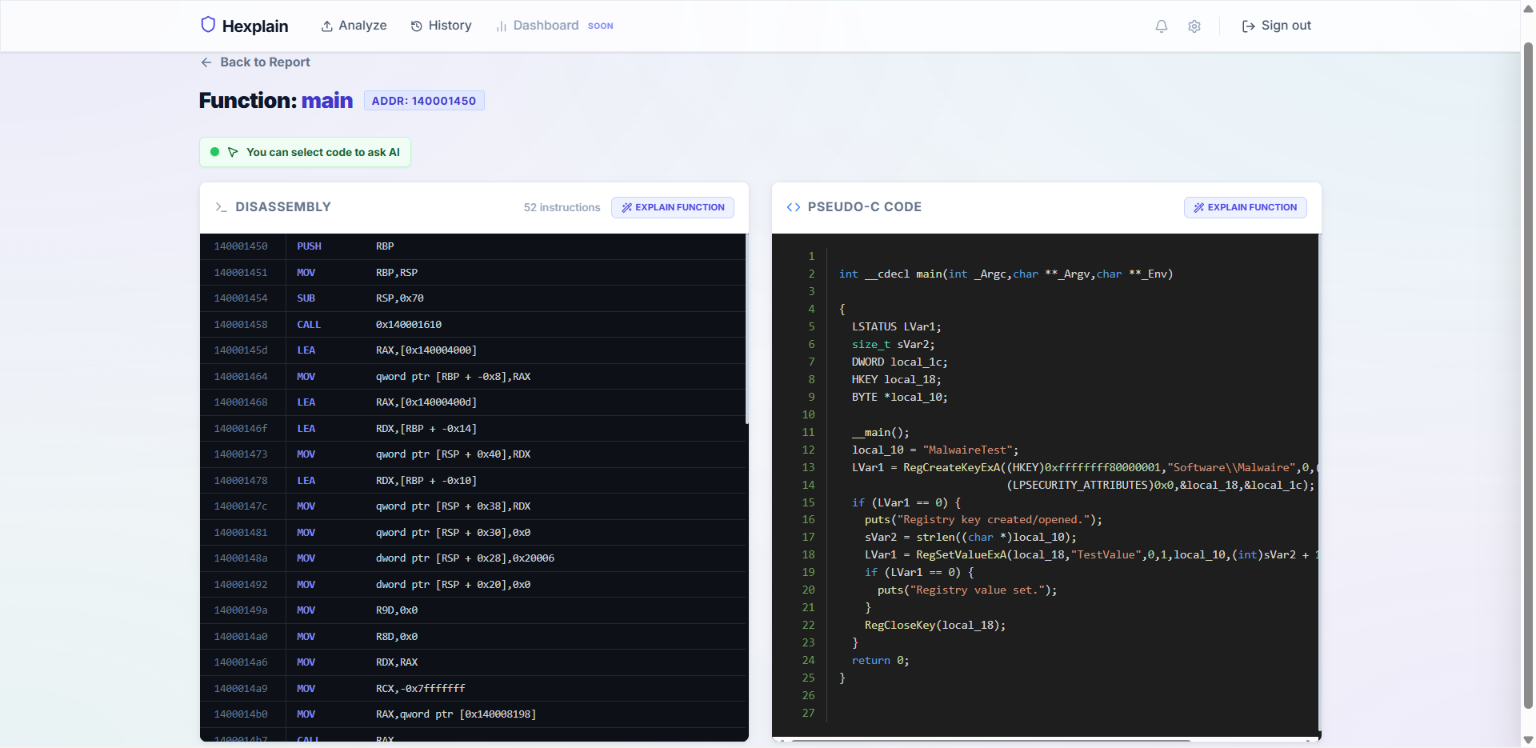
\includegraphics[width=\textwidth]{function_disassembly_pseudocode}
  \caption{Vue désassembleur (gauche) et pseudo-C Ghidra (droite) d'une fonction de manipulation de registre Windows --- illustrant la complexité de l'assembleur pour un non-expert}
  \label{fig:function_disassembly}
\end{figure}

Des études menées dans le domaine de l'enseignement de la rétro-ingénierie~\cite{eagle2011ghidra} montrent qu'il faut en moyenne \textbf{18 à 24 mois} de pratique intensive pour qu'un ingénieur logiciel puisse analyser des binaires complexes avec autonomie. Cette durée d'apprentissage est incompatible avec les délais de réponse aux incidents de sécurité.

\subsubsection{La fragmentation des outils}

Un analyste qui souhaite réaliser une analyse complète d'un binaire doit aujourd'hui~:
\begin{enumerate}
  \item Ouvrir Ghidra pour désassembler et décompiler le code.
  \item Exécuter YARA en ligne de commande pour tester les règles de signatures.
  \item Lancer Capa sur le fichier pour obtenir les capacités MITRE.
  \item Uploader le hash sur VirusTotal via son navigateur web.
  \item Agréger manuellement les résultats dans un rapport Word ou Excel.
\end{enumerate}

Ce processus, outre son coût en temps, est source d'erreurs et de pertes d'informations lors de la consolidation manuelle. Aucun outil existant n'offre une vision unifiée et corrélée de l'ensemble de ces informations~\cite{ligh2010malware}.

\subsubsection{L'absence de contextualisation et d'explication}

Les outils actuels produisent des données brutes~: une liste d'imports, un score VirusTotal, des identifiants de règles YARA, des techniques MITRE ATT\&CK. Ces informations sont précieuses pour l'expert, mais \textbf{totalement opaques pour l'analyste novice} qui ne sait pas ce que signifie concrètement «~T1055 - Process Injection~» ou «~L'entropie de la section .rsrc est de 7.95~». L'absence de couche d'explication pédagogique constitue une barrière à l'adoption de ces outils par des équipes non spécialisées.

\subsubsection{Le coût temporel et humain}

Selon les experts du domaine~\cite{sikorski2012practical}, l'analyse complète d'un malware de complexité moyenne peut prendre de \textbf{4 à 8 heures} pour un analyste expérimenté. Pour un binaire obfusqué ou packé, ce délai peut dépasser plusieurs jours. Dans un contexte d'incident de sécurité critique, ce délai est souvent inacceptable. Les équipes SOC (\textit{Security Operations Center}) sous-staffées ont besoin d'outils capables de fournir une première évaluation rapide et fiable, permettant de trier et prioriser les menaces.

\subsubsection{Solutions commerciales~: accessibles mais coûteuses}

Des solutions commerciales comme \textbf{Intezer Analyze}, \textbf{Joe Sandbox} ou \textbf{Recorded Future} proposent des analyses automatisées de haute qualité, mais à des tarifs annuels inaccessibles pour les PME, les équipes académiques ou les pays en développement. Il existe donc un \textbf{vide entre les outils gratuits complexes et les solutions commerciales hors de portée}.

\section{Présentation du projet Hexplain}

\subsection{Enjeux et vision}

\textbf{Hexplain} (contraction de «~Hex Explain~», en référence aux dump hexadécimaux que les analystes déchiffrent au quotidien) est une plateforme open-source d'analyse statique de binaires PE/ELF/.NET assistée par intelligence artificielle. Sa vision fondamentale est de \textbf{démocratiser la compréhension des malwares}~: rendre accessible à un analyste junior ou à une équipe sans ressources spécialisées des analyses qui requièrent aujourd'hui des années d'expertise.

\subsection{Solution proposée et valeurs ajoutées}

Hexplain répond aux lacunes identifiées ci-dessus par plusieurs innovations complémentaires~:

\begin{enumerate}
  \item \textbf{Pipeline unifié en 9 étapes}~: En un seul upload, l'utilisateur déclenche automatiquement l'ensemble de la chaîne d'analyse (métadonnées, YARA, Capa, Ghidra, threat intel, scoring), sans configuration ni expertise préalable.

  \item \textbf{Génération de rapports en langage naturel (LLM)}~: Un modèle de langage (Gemini 2.0 Flash ou Llama-3.1) analyse les sorties brutes du pipeline et les traduit en explications pédagogiques structurées~: résumé exécutif, comportements clés, explications des techniques MITRE, analyse fonction par fonction. L'\textbf{hallucination est explicitement prévenue} par des garde-fous stricts dans les prompts~: le modèle est instruit de ne jamais affirmer une classification qu'il ne peut corroborer par des preuves multiples et concrètes.

  \item \textbf{Score de risque hybride}~: La plateforme calcule un score de risque sur 100 points combinant une composante heuristique déterministe (basée sur des règles pondérées) et une composante LLM contextuelle. Cette double approche réduit les faux positifs et les faux négatifs.

  \item \textbf{Chatbot RAG pédagogique}~: L'utilisateur peut, après avoir reçu son rapport, poser des questions en langage naturel sur le binaire analysé (<<~Que fait la fonction à l'adresse 0x401000~?~>>, <<~Pourquoi le score de risque est-il aussi élevé~?~>>). Le système RAG local garantit que les réponses sont ancrées exclusivement dans les données du rapport, sans fabrication d'informations.

  \item \textbf{Sécurité native}~: La conception sécurité-d'abord est une différenciation majeure~: les fichiers malveillants sont isolés en quarantaine (volume non-servi, permissions \texttt{0o440}), jamais exécutés, et tous les accès sont protégés par authentification forte et CSRF.

  \item \textbf{Accessibilité économique}~: La solution fonctionne sur des APIs gratuites (Groq, Gemini, VirusTotal free tier) et peut être déployée sur un serveur modeste (DigitalOcean Droplet à faible coût), rendant la cybersécurité avancée accessible aux organisations à ressources limitées.
\end{enumerate}

\subsection{Périmètre du projet}

Dans le cadre de ce stage (8 semaines), le projet a été développé en \textbf{quatre sprints itératifs}~:

\begin{table}[H]
  \centering
  \caption{Sprints de développement du projet Hexplain}
  \label{tab:sprints}
  \begin{tabularx}{\textwidth}{c X l}
    \toprule
    \textbf{Sprint} & \textbf{Périmètre} & \textbf{Statut} \\
    \midrule
    1 & Fondation sécurisée~: authentification (Argon2id, JWT, CSRF), upload et quarantaine des fichiers, file de tâches asynchrones (Celery/Redis) & \textcolor{successgreen}{\textbf{Terminé}} \\
    \midrule
    2 & Moteur d'analyse statique~: parsing PE/ELF, YARA, Capa, Ghidra/ILSpy, threat intelligence (VT, MalwareBazaar, OTX), scoring heuristique & \textcolor{successgreen}{\textbf{Terminé}} \\
    \midrule
    3 & Couche LLM/RAG~: génération de rapport LLM (Groq/Gemini), pipeline RAG local (ChromaDB + sentence-transformers), chatbot multi-sessions & \textcolor{successgreen}{\textbf{Terminé}} \\
    \midrule
    4 & Frontend dashboard complet (Next.js), export PDF, déploiement DigitalOcean, pipeline CI/CD GitHub Actions & \textcolor{successgreen}{\textbf{Terminé}} \\
    \bottomrule
  \end{tabularx}
\end{table}

\section{Démarche méthodologique adoptée}

\subsection{Approche itérative par sprints}

La méthodologie de développement adoptée s'inspire des pratiques agiles~: le projet a été découpé en \textbf{sprints de deux semaines} chacun, avec des objectifs clairs, des livrables définis et des points de validation réguliers avec l'encadrant professionnel. Cette approche a permis de détecter et corriger rapidement les dérives techniques (notamment lors de l'intégration de Ghidra dans un conteneur Docker), et d'ajuster les priorités en fonction des retours de validation.

\subsection{Principe de sécurité par conception}

Dès la conception du système, le principe \textit{security by design} a été appliqué de manière systématique~: chaque fonctionnalité a été évaluée selon son impact potentiel sur la sécurité avant toute implémentation. Ce principe s'est traduit notamment par~:
\begin{itemize}
  \item L'isolation physique des fichiers malveillants dans un volume Docker non-servi.
  \item La validation en deux passes des fichiers uploadés (magic bytes bruts + libmagic).
  \item L'utilisation de listes d'autorisation strictes (PE/ELF uniquement).
  \item L'absence de toute exécution des binaires analysés à quelque étape que ce soit du pipeline.
\end{itemize}

\subsection{Modularité et résilience du pipeline}

Le pipeline d'analyse a été conçu selon un principe de \textbf{résilience modulaire}~: chaque module d'analyse est enveloppé dans un gestionnaire d'erreurs isolé (\texttt{\_safe\_call}). Si un module échoue (Ghidra qui dépasse son timeout, VirusTotal qui renvoie une erreur HTTP), le pipeline continue son exécution avec les modules restants et préserve les résultats partiels. Cela garantit qu'une défaillance ponctuelle ne prive pas l'utilisateur de l'ensemble des informations disponibles.

\section{Outils et technologies utilisés}

\subsection{Backend et analyse statique}

\begin{table}[H]
  \centering
  \caption{Technologies backend et analyse statique}
  \label{tab:tech_backend}
  \begin{tabularx}{\textwidth}{l l X}
    \toprule
    \textbf{Technologie} & \textbf{Version} & \textbf{Rôle} \\
    \midrule
    FastAPI & $\geq$ 0.115 & Framework web Python asynchrone pour l'API REST \\
    Celery & $\geq$ 5.4 & File de tâches asynchrones pour l'exécution du pipeline \\
    Redis & 7-alpine & Broker de messages et backend de résultats Celery \\
    SQLite (SQLAlchemy) & $\geq$ 2.0 & Base de données relationnelle avec ORM \\
    Alembic & $\geq$ 1.13 & Gestion des migrations de schéma de base de données \\
    LIEF & $\geq$ 0.16 & Parsing des structures PE/ELF (sections, imports, entropie) \\
    pefile & $\geq$ 2023.2 & Parsing complémentaire du format PE \\
    pyelftools & $\geq$ 0.31 & Parsing du format ELF \\
    capstone & $\geq$ 5.0 & Moteur de désassemblage (x86/x64/ARM) \\
    yara-python & $\geq$ 4.5 & Binding Python pour le moteur YARA \\
    flare-capa & $\geq$ 9.0 & Détection de capacités et mapping MITRE ATT\&CK \\
    Ghidra & 11.x & Décompilateur headless pour binaires natifs C/C++ \\
    ilspycmd & \textemdash & Décompilateur CLI pour binaires .NET (C\#) \\
    python-magic & $\geq$ 0.4.27 & Détection de type par magic bytes \\
    argon2-cffi & $\geq$ 23.1 & Hachage de mots de passe Argon2id \\
    python-jose & $\geq$ 3.3 & Génération et validation des JWT \\
    slowapi & $\geq$ 0.1.9 & Limitation de débit (rate limiting) sur les endpoints \\
    structlog & $\geq$ 24.0 & Journalisation structurée en JSON \\
    \bottomrule
  \end{tabularx}
\end{table}

\subsection{LLM et RAG}

\begin{table}[H]
  \centering
  \caption{Technologies LLM et RAG}
  \label{tab:tech_llm}
  \begin{tabularx}{\textwidth}{l X}
    \toprule
    \textbf{Technologie} & \textbf{Rôle} \\
    \midrule
    Google Gemini 2.0 Flash & Fournisseur LLM principal~: génération de rapports et réponses RAG \\
    Groq API (Llama-3.1-8b-instant) & Fournisseur LLM secondaire~: basculement automatique si Gemini indisponible \\
    ChromaDB ($\geq$ 0.4) & Base de données vectorielle locale pour le système RAG \\
    sentence-transformers ($\geq$ 2.0) & Génération d'embeddings sémantiques (modèle all-MiniLM-L6-v2) \\
    googlesearch-python & Recherche OSINT DuckDuckGo pour l'enrichissement IA des IOC \\
    \bottomrule
  \end{tabularx}
\end{table}

\subsection{Frontend et déploiement}

\begin{table}[H]
  \centering
  \caption{Technologies frontend et infrastructure}
  \label{tab:tech_frontend}
  \begin{tabularx}{\textwidth}{l l X}
    \toprule
    \textbf{Technologie} & \textbf{Version} & \textbf{Rôle} \\
    \midrule
    Next.js & 14 & Framework React pour le frontend avec rendu SSR/SSG \\
    TypeScript & \textemdash & Typage statique du code JavaScript \\
    Tailwind CSS & \textemdash & Framework CSS utilitaire pour le styling \\
    @react-pdf/renderer & \textemdash & Génération de rapports PDF côté navigateur \\
    Docker & 24+ & Containerisation des services \\
    Docker Compose & v2+ & Orchestration multi-conteneurs \\
    DigitalOcean Droplet & Ubuntu & Hébergement de la plateforme en production \\
    GitHub Actions & \textemdash & Pipeline CI/CD automatisé (SCP + SSH deploy) \\
    \bottomrule
  \end{tabularx}
\end{table}

\section{Conclusion}

Ce chapitre a mis en lumière les lacunes fondamentales des approches actuelles d'analyse statique de malwares~: barrière de compétence en assembleur, fragmentation des outils, absence d'explication pédagogique et coûts temporels prohibitifs. Face à ces problèmes bien identifiés, le projet Hexplain propose une réponse intégrée, combinant un pipeline d'analyse complet, une couche LLM explicative et un chatbot RAG contextuel, le tout dans une architecture sécurisée et déployable à faible coût. Le chapitre suivant présente l'analyse des besoins formalisée et les diagrammes de conception qui ont guidé le développement du système.

% =============================================================================
% Chapitre 3 — Analyse et Conception
% =============================================================================

\chapter{Analyse et Conception}

\section{Introduction}

La phase d'analyse et de conception constitue le fondement de tout projet logiciel rigoureux. Elle permet de formaliser les exigences du système, de définir les acteurs et leurs interactions, et de produire les artefacts de modélisation qui guideront l'implémentation. Ce chapitre présente successivement l'analyse des besoins fonctionnels et non fonctionnels, les diagrammes de cas d'utilisation, les diagrammes de séquence des scénarios clés, et le modèle de données sous forme de diagramme de classes.

\section{Analyse des besoins}

\subsection{Besoins fonctionnels}

Les besoins fonctionnels décrivent les fonctions que le système doit réaliser du point de vue de l'utilisateur. Ils ont été identifiés lors de la phase d'analyse initiale en collaboration avec l'encadrant professionnel.

\subsubsection{Module d'authentification et de gestion des utilisateurs}
\begin{itemize}
  \item \textbf{BF-01}~: Le système doit permettre à un utilisateur de créer un compte avec email, nom d'utilisateur et mot de passe.
  \item \textbf{BF-02}~: Le système doit authentifier les utilisateurs par identifiant et mot de passe, et maintenir la session via un JWT stocké dans un cookie HttpOnly.
  \item \textbf{BF-03}~: Le système doit permettre la déconnexion sécurisée (suppression du cookie de session).
  \item \textbf{BF-04}~: Chaque utilisateur ne doit avoir accès qu'à ses propres analyses (isolation par \texttt{user\_id}).
\end{itemize}

\subsubsection{Module de soumission et de gestion des fichiers}
\begin{itemize}
  \item \textbf{BF-05}~: Le système doit accepter l'upload de fichiers binaires PE (Windows), ELF (Linux) et .NET assemblies.
  \item \textbf{BF-06}~: Le système doit valider le type du fichier par magic bytes avant tout traitement.
  \item \textbf{BF-07}~: Le système doit stocker les fichiers dans un volume de quarantaine isolé, jamais servi directement.
  \item \textbf{BF-08}~: Le système doit calculer les empreintes SHA-256, SHA-1 et MD5 du fichier uploadé.
  \item \textbf{BF-09}~: Le système doit lancer automatiquement l'analyse après l'upload et retourner immédiatement un \texttt{job\_id}.
\end{itemize}

\subsubsection{Module de pipeline d'analyse statique}
\begin{itemize}
  \item \textbf{BF-10}~: Le pipeline doit extraire les métadonnées du fichier (architecture, entropie, signature numérique, compilateur).
  \item \textbf{BF-11}~: Le pipeline doit parser la structure PE/ELF (sections, imports, exports) et détecter les sections à haute entropie (potentiellement packées ou chiffrées).
  \item \textbf{BF-12}~: Le pipeline doit identifier les API Windows suspectes utilisées par le binaire (injection, persistance, réseau, cryptographie).
  \item \textbf{BF-13}~: Le pipeline doit extraire les chaînes de caractères imprimables et filtrer les IOC (URLs, adresses IP, chemins de fichiers, clés de registre).
  \item \textbf{BF-14}~: Le pipeline doit scanner le fichier avec des règles YARA communautaires et personnalisées.
  \item \textbf{BF-15}~: Le pipeline doit analyser les capacités du binaire via Mandiant Capa et les mapper sur MITRE ATT\&CK.
  \item \textbf{BF-16}~: Le pipeline doit décompiler le binaire via Ghidra (natif) ou ILSpy (pour .NET) et extraire les fonctions clés.
  \item \textbf{BF-17}~: Le pipeline doit interroger les plateformes de threat intelligence (VirusTotal, MalwareBazaar, AlienVault OTX) par hash.
  \item \textbf{BF-18}~: Le pipeline doit calculer un score de risque heuristique sur 100 points et attribuer un niveau de risque (clean, low, medium, high, critical).
\end{itemize}

\subsubsection{Module LLM et RAG}
\begin{itemize}
  \item \textbf{BF-19}~: Le système doit générer un rapport d'analyse en langage naturel via un LLM, incluant résumé exécutif, classification, comportements clés, explications MITRE et analyse des fonctions décompilées.
  \item \textbf{BF-20}~: Le système doit calculer un score de risque LLM combiné au score heuristique.
  \item \textbf{BF-21}~: Le système doit indexer le rapport dans une base vectorielle locale (ChromaDB) pour permettre les requêtes RAG.
  \item \textbf{BF-22}~: L'utilisateur doit pouvoir poser des questions en langage naturel sur le rapport, auxquelles le chatbot RAG répondra exclusivement sur la base du contenu indexé.
  \item \textbf{BF-23}~: Le système doit gérer des sessions de chat persistantes (multi-tours) avec historique des échanges.
\end{itemize}

\subsubsection{Module de restitution et d'export}
\begin{itemize}
  \item \textbf{BF-24}~: L'utilisateur doit pouvoir consulter l'historique de toutes ses analyses avec leur statut et score de risque.
  \item \textbf{BF-25}~: L'utilisateur doit pouvoir suivre en temps réel l'avancement de l'analyse (10 étapes avec statut visuel).
  \item \textbf{BF-26}~: Le rapport doit être navigable par sections (fonctions, sections binaires, IOC, capacités, facteurs de risque).
  \item \textbf{BF-27}~: L'utilisateur doit pouvoir exporter le rapport au format PDF ou JSON.
  \item \textbf{BF-28}~: L'utilisateur doit pouvoir demander une explication contextuelle par IA sur n'importe quel élément du rapport (section, fonction, facteur de risque).
\end{itemize}

\subsection{Besoins non fonctionnels}

\subsubsection{Sécurité (priorité maximale)}
\begin{itemize}
  \item \textbf{BNF-01}~: Aucun fichier uploadé ne doit être exécuté à quelque étape que ce soit du traitement.
  \item \textbf{BNF-02}~: Les mots de passe doivent être hachés avec Argon2id (résistant aux attaques GPU).
  \item \textbf{BNF-03}~: Toutes les requêtes modifiant l'état doivent être protégées contre les attaques CSRF.
  \item \textbf{BNF-04}~: Les clés API externes ne doivent jamais apparaître dans les réponses API ni dans les journaux d'erreurs.
  \item \textbf{BNF-05}~: Les appels de sous-processus doivent utiliser des listes d'arguments (interdiction de \texttt{shell=True}).
  \item \textbf{BNF-06}~: La sérialisation Celery doit utiliser JSON uniquement (interdiction de pickle).
\end{itemize}

\subsubsection{Performance et disponibilité}
\begin{itemize}
  \item \textbf{BNF-07}~: L'API doit répondre aux requêtes de consultation en moins de 500~ms.
  \item \textbf{BNF-08}~: L'upload d'un fichier doit être accepté (202 Accepted) en moins de 2 secondes.
  \item \textbf{BNF-09}~: L'analyse complète d'un binaire de taille standard (< 10 MB) doit s'achever en moins de 5 minutes.
  \item \textbf{BNF-10}~: Le chatbot RAG doit retourner une réponse en moins de 10 secondes.
\end{itemize}

\subsubsection{Maintenabilité et extensibilité}
\begin{itemize}
  \item \textbf{BNF-11}~: Le pipeline d'analyse doit être extensible~: l'ajout d'un nouveau module ne doit pas modifier les modules existants.
  \item \textbf{BNF-12}~: La configuration doit être externalisée dans des variables d'environnement (fichier \texttt{.env}).
  \item \textbf{BNF-13}~: Le code doit être documenté avec des docstrings et des commentaires explicatifs.
\end{itemize}

\subsubsection{Accessibilité économique}
\begin{itemize}
  \item \textbf{BNF-14}~: La solution doit fonctionner avec des APIs gratuites ou à faible coût.
  \item \textbf{BNF-15}~: En l'absence de clé API LLM, le pipeline d'analyse statique doit continuer à fonctionner de manière dégradée (sans couche LLM).
\end{itemize}

\subsection{Exigences techniques}

\begin{itemize}
  \item Architecture microservices containerisée (Docker Compose).
  \item Base de données SQLite compatible avec une migration future vers PostgreSQL.
  \item Frontend Next.js compilable en production sur un serveur Node.js.
  \item Compatibilité avec les environnements WSL2 + Docker Desktop (Windows).
\end{itemize}

\section{Modélisation fonctionnelle --- Diagrammes de cas d'utilisation}

Le diagramme de cas d'utilisation présenté en Figure~\ref{fig:use_case} identifie les trois acteurs principaux du système et leurs interactions avec les fonctionnalités offertes.

\begin{figure}[H]
  \centering
  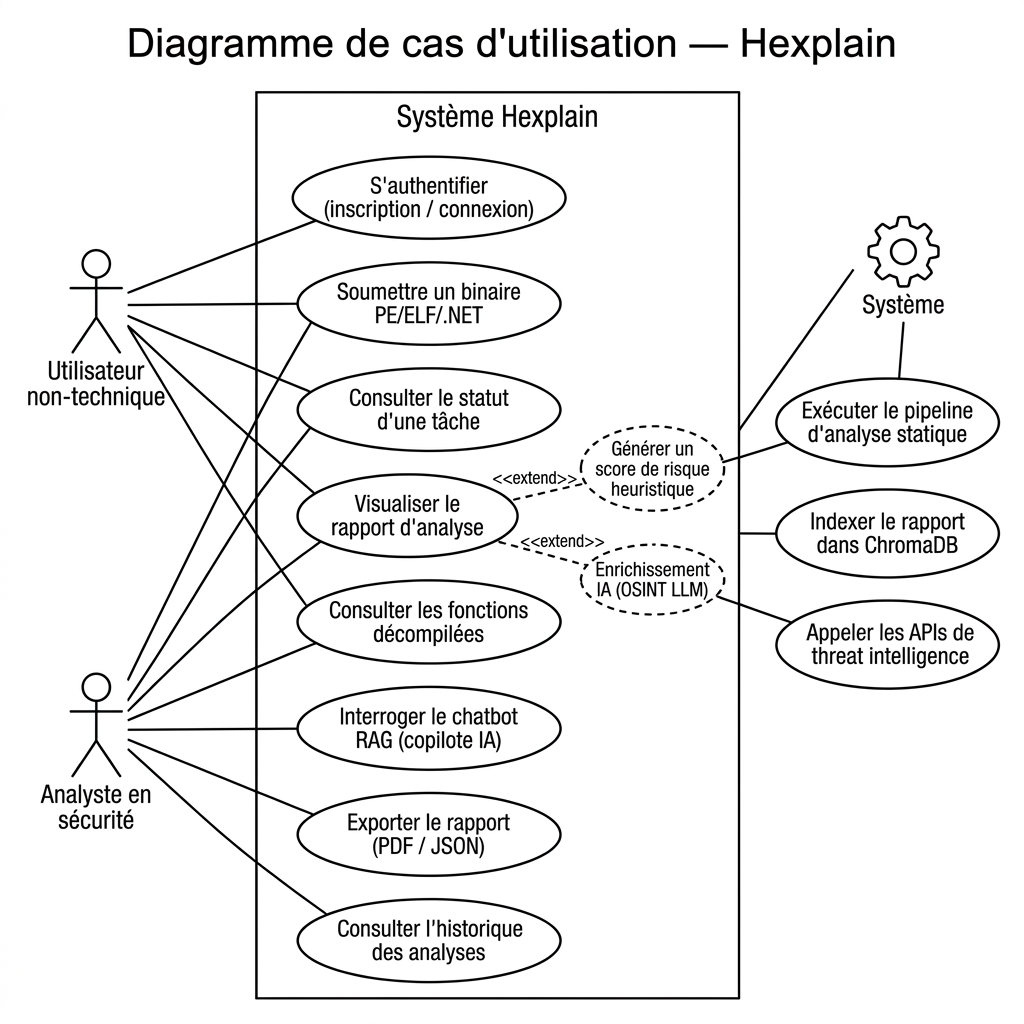
\includegraphics[width=0.9\textwidth]{diagramme_cas_utilisation}
  \caption{Diagramme de cas d'utilisation global --- Hexplain}
  \label{fig:use_case}
\end{figure}

\subsection{Description des acteurs}

\begin{description}
  \item[\textbf{Utilisateur non-technique}] Toute personne souhaitant analyser un fichier suspect sans expertise en rétro-ingénierie. Il accède aux fonctionnalités de base~: upload, consultation du rapport, chat avec le copilote IA et export.

  \item[\textbf{Analyste en sécurité}] Expert en cybersécurité souhaitant accélérer son workflow. Il utilise les mêmes fonctionnalités que l'utilisateur non-technique, en y ajoutant la consultation détaillée des fonctions décompilées et l'interprétation avancée des IOC et des techniques MITRE.

  \item[\textbf{Système}] Acteur interne représentant les services automatiques~: exécution du pipeline d'analyse, indexation du rapport dans ChromaDB, appels aux APIs de threat intelligence. Ces actions sont déclenchées sans intervention directe de l'utilisateur.
\end{description}

\subsection{Cas d'utilisation étendus}

Deux cas d'utilisation étendent \textit{Visualiser le rapport d'analyse} via la relation \texttt{<<extend>>}~:
\begin{itemize}
  \item \textbf{Générer un score de risque heuristique}~: déclenché automatiquement à la fin du pipeline, il calcule et stocke le score composite.
  \item \textbf{Enrichissement IA (OSINT LLM)}~: déclenché conditionnellement lorsque le score heuristique est élevé mais que le threat intelligence ne remonte pas de correspondances précises.
\end{itemize}

\section{Conception technique --- Diagrammes de séquence}

\subsection{Scénario 1~: Analyse complète d'un binaire PE/ELF}

Le diagramme de séquence de la Figure~\ref{fig:seq_analyse} illustre le flux complet d'une analyse de binaire, depuis l'upload jusqu'à la restitution du rapport final.

\begin{figure}[H]
  \centering
  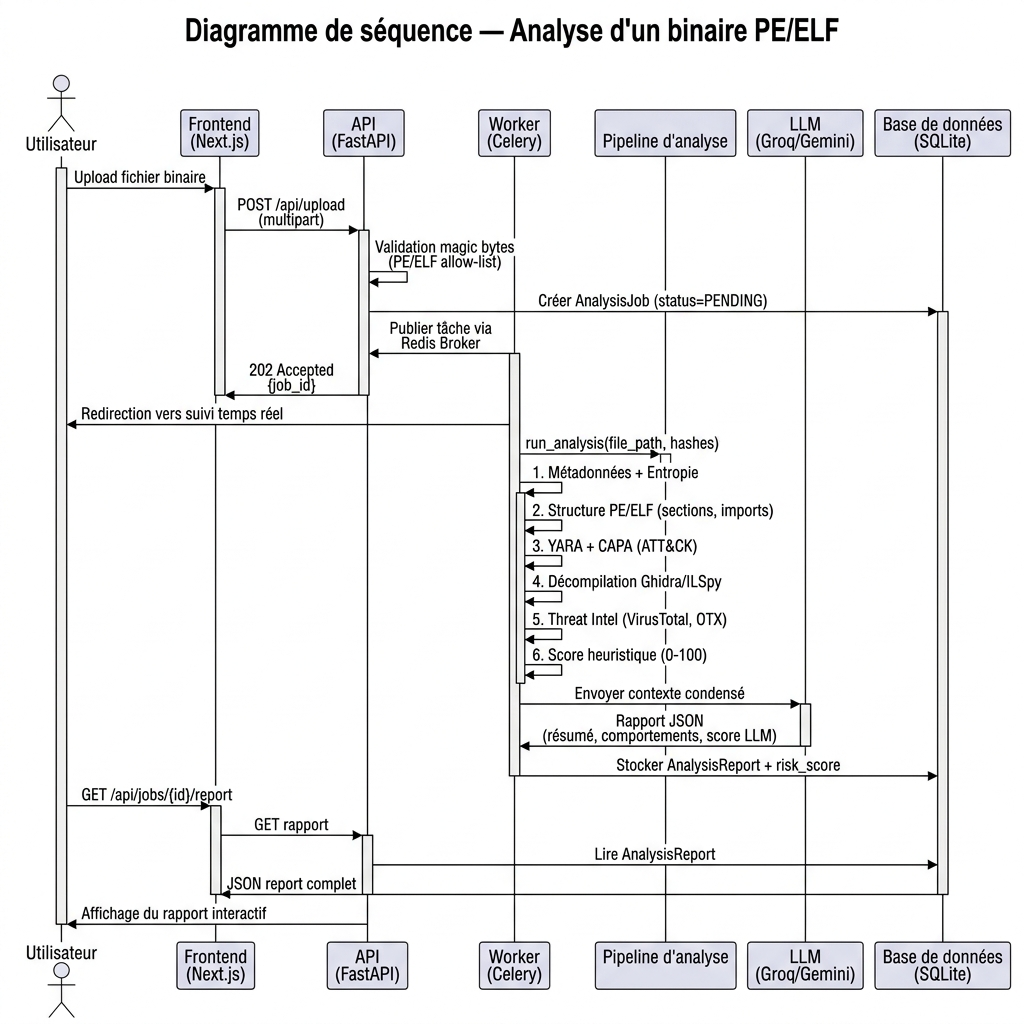
\includegraphics[width=\textwidth]{diagramme_sequence_analyse}
  \caption{Diagramme de séquence --- Analyse complète d'un binaire PE/ELF}
  \label{fig:seq_analyse}
\end{figure}

Les points clés de ce scénario sont~:
\begin{enumerate}
  \item \textbf{Acceptation immédiate}~: L'API retourne un \texttt{202 Accepted} avec le \texttt{job\_id} dès réception du fichier validé, sans attendre la fin de l'analyse. Ce pattern asynchrone permet à l'interface de proposer un suivi en temps réel.
  \item \textbf{Isolation de la quarantaine}~: Le Worker accède au fichier directement dans le volume monté (\texttt{/app/quarantine}), sans que l'API n'ait à transmettre le contenu du fichier via le broker Redis.
  \item \textbf{Résilience modulaire}~: Chaque étape du pipeline est isolée dans un wrapper \texttt{\_safe\_call}. Une défaillance d'un module (timeout Ghidra, erreur réseau VirusTotal) n'interrompt pas le pipeline.
  \item \textbf{Double scoring}~: Le score heuristique est calculé à partir des sorties déterministes du pipeline, puis affiné par le LLM qui produit son propre score contextuel. Le score final combiné est stocké dans \texttt{AnalysisReport.risk\_score}.
\end{enumerate}

\subsection{Scénario 2~: Flux RAG (interrogation du chatbot)}

Le diagramme de séquence de la Figure~\ref{fig:seq_rag} détaille le mécanisme de Retrieval-Augmented Generation qui permet au chatbot de répondre aux questions de l'utilisateur de manière contextuellement ancrée.

\begin{figure}[H]
  \centering
  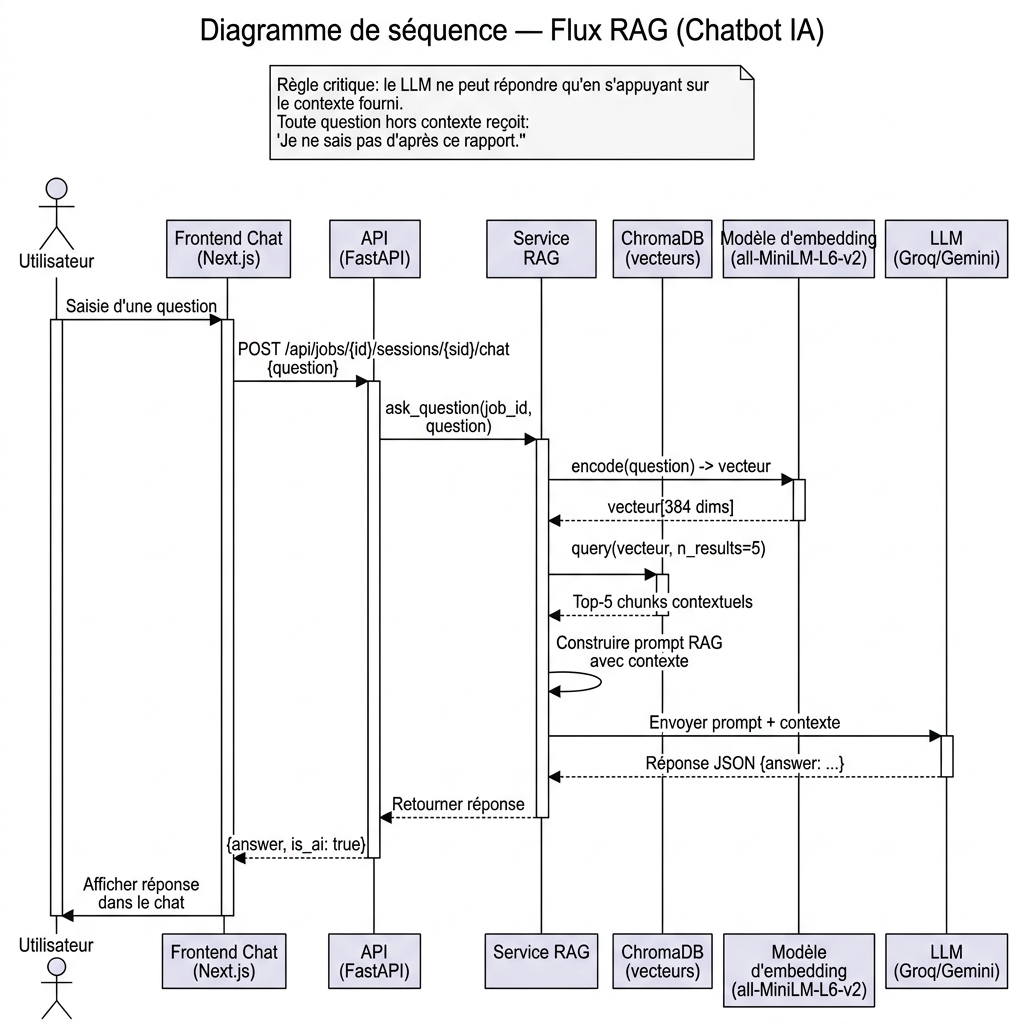
\includegraphics[width=\textwidth]{diagramme_sequence_rag}
  \caption{Diagramme de séquence --- Flux RAG (chatbot pédagogique)}
  \label{fig:seq_rag}
\end{figure}

Les étapes clés de ce flux sont~:
\begin{enumerate}
  \item \textbf{Embedding de la question}~: La question de l'utilisateur est encodée en un vecteur de 384 dimensions par le modèle \textit{all-MiniLM-L6-v2} localement (sans appel API externe).
  \item \textbf{Retrieval sémantique}~: ChromaDB recherche les 5 chunks les plus sémantiquement proches parmi ceux indexés lors de la génération du rapport (résumé, comportements, fonctions, techniques MITRE).
  \item \textbf{Génération ancrée}~: Le LLM reçoit uniquement ces 5 chunks comme contexte, avec une instruction stricte~: répondre exclusivement sur la base de ce contexte ou déclarer explicitement l'impossibilité de répondre. Ce mécanisme prévient l'hallucination.
\end{enumerate}

\section{Modélisation des données --- Diagramme de classes}

Le diagramme de classes de la Figure~\ref{fig:class_diagram} présente le modèle de données relationnel de Hexplain, tel qu'il est implémenté avec SQLAlchemy (ORM Python).

\begin{figure}[H]
  \centering
  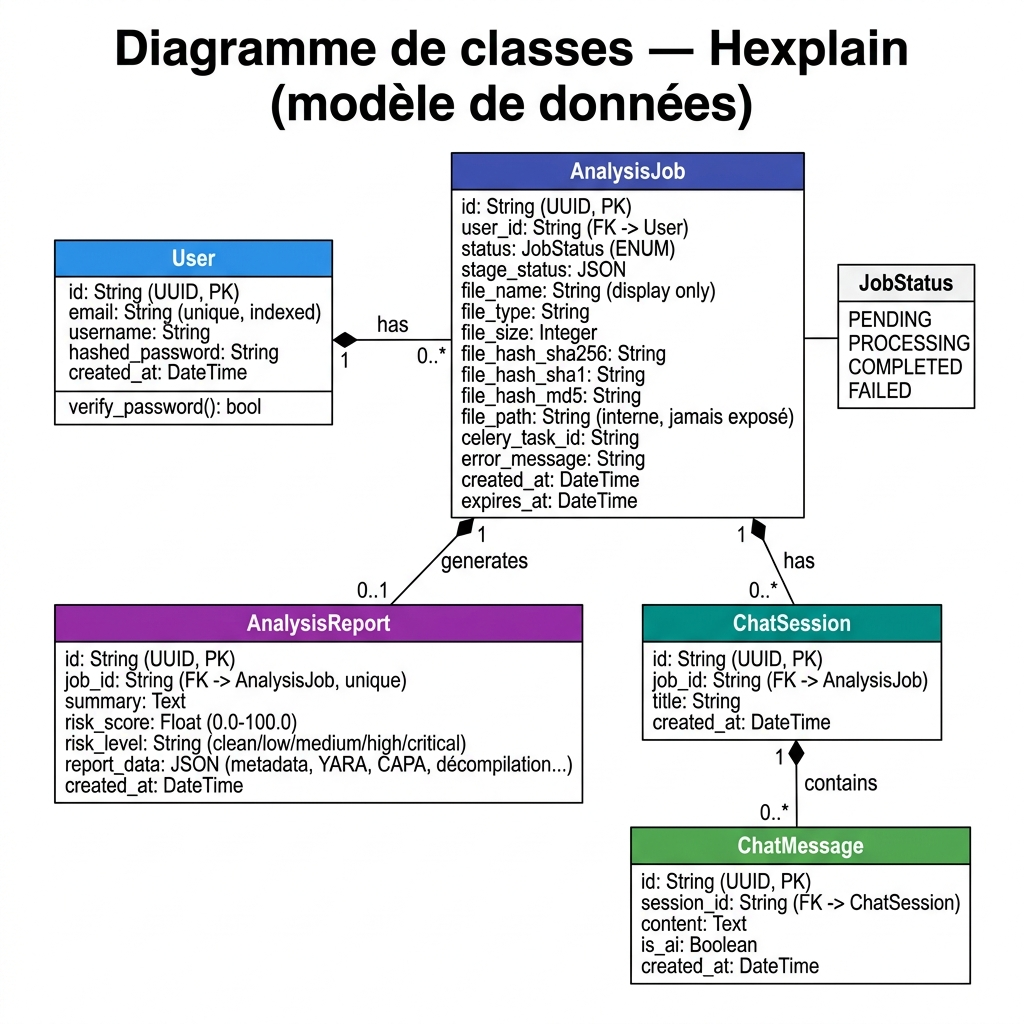
\includegraphics[width=0.95\textwidth]{diagramme_classes}
  \caption{Diagramme de classes --- Modèle de données Hexplain}
  \label{fig:class_diagram}
\end{figure}

\subsection{Description des entités}

\begin{description}
  \item[\textbf{User}] Représente un compte utilisateur. L'attribut \texttt{hashed\_password} stocke le hash Argon2id du mot de passe (jamais le mot de passe en clair). La méthode \texttt{verify\_password()} compare un mot de passe soumis à son hash stocké via le contexte Argon2id.

  \item[\textbf{AnalysisJob}] Entité centrale du système. Chaque job correspond à un fichier uploadé et suit un cycle de vie~: \texttt{PENDING} $\rightarrow$ \texttt{PROCESSING} $\rightarrow$ \texttt{COMPLETED}/\texttt{FAILED}. L'attribut \texttt{file\_path} stocke l'emplacement physique du fichier en quarantaine~: il est interne au système et \textbf{ne doit jamais être exposé dans les réponses API}. Les trois attributs de hash (SHA-256, SHA-1, MD5) permettent la déduplication et les lookups de threat intelligence.

  \item[\textbf{AnalysisReport}] Stocke les résultats de l'analyse~: score de risque (\texttt{risk\_score}, 0-100), niveau de risque (\texttt{risk\_level}) et le blob JSON complet (\texttt{report\_data}) contenant toutes les sorties du pipeline. La relation avec \texttt{AnalysisJob} est de type one-to-one avec cascade de suppression.

  \item[\textbf{ChatSession}] Représente une session de conversation multi-tours associée à un job. Un job peut avoir plusieurs sessions de chat indépendantes, permettant à l'utilisateur d'organiser ses interrogations par thème.

  \item[\textbf{ChatMessage}] Stocke chaque message d'une session de chat. L'attribut \texttt{is\_ai} distingue les messages utilisateur des réponses générées par le LLM/RAG.

  \item[\textbf{JobStatus (Enum)}] Définit les quatre états possibles du cycle de vie d'un job~: \texttt{PENDING} (en attente de traitement), \texttt{PROCESSING} (analyse en cours), \texttt{COMPLETED} (analyse réussie), \texttt{FAILED} (erreur irrémédiable).
\end{description}

\subsection{Règles métier importantes}

\begin{itemize}
  \item \textbf{Isolation par utilisateur}~: Toutes les requêtes sur \texttt{AnalysisJob} et \texttt{AnalysisReport} filtrent systématiquement par \texttt{user\_id}. Un utilisateur ne peut jamais accéder aux données d'un autre utilisateur.
  \item \textbf{Expiration automatique}~: L'attribut \texttt{expires\_at} (par défaut, 7 jours après la création) permet une politique de rétention et de nettoyage automatique des fichiers.
  \item \textbf{Cascade de suppression}~: La suppression d'un \texttt{User} entraîne la suppression de tous ses jobs, rapports, sessions et messages en cascade.
\end{itemize}

\section{Conclusion}

Ce chapitre a formalisé l'ensemble des exigences du système Hexplain à travers une analyse structurée des besoins fonctionnels, non fonctionnels et techniques. Les diagrammes UML produits --- cas d'utilisation, séquences et classes --- constituent les artefacts de référence qui ont guidé l'implémentation. Ils montrent notamment la séparation claire des responsabilités entre l'API, le Worker asynchrone et le service RAG, ainsi que la rigueur du modèle de données en matière de sécurité (isolation par utilisateur, champs internes jamais exposés). Le chapitre suivant entre dans les détails de l'architecture technique du pipeline.

% =============================================================================
% Chapitre 4 — Architecture et aspects techniques
% =============================================================================

\chapter{Architecture et aspects techniques}

\section{Introduction}

Ce chapitre présente l'architecture technique détaillée de la plateforme Hexplain. Après une vue d'ensemble de l'architecture globale, nous décrirons chaque module du pipeline d'analyse, l'infrastructure Docker et l'orchestration des services, les mécanismes de sécurité mis en œuvre, et les flux de communication entre composants. Ce chapitre est le cœur technique du rapport~: il s'appuie directement sur le code source développé pendant le stage.

\section{Architecture globale du pipeline}

\subsection{Vue d'ensemble}

Hexplain repose sur une architecture \textbf{microservices conteneurisée} orchestrée par Docker Compose. Quatre conteneurs collaborent pour offrir l'ensemble des fonctionnalités de la plateforme~:

\begin{figure}[H]
  \centering
  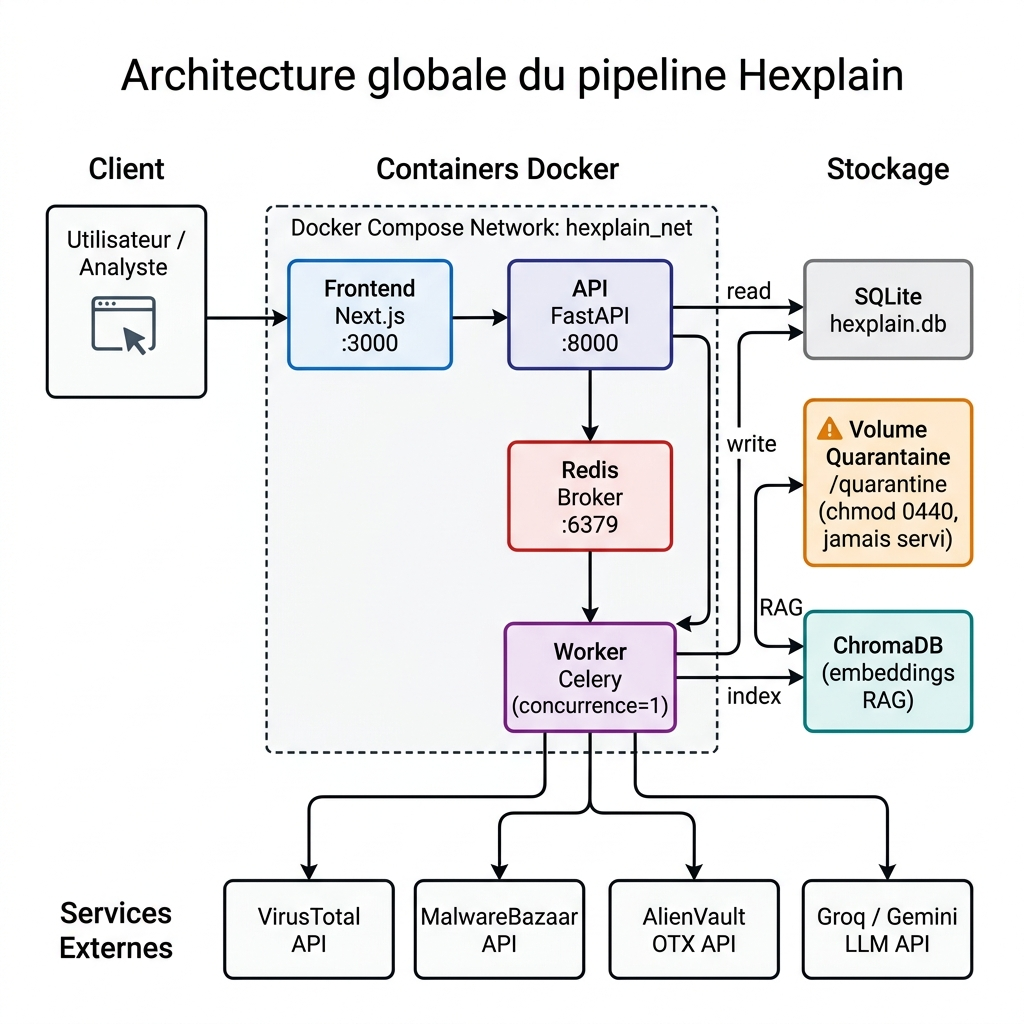
\includegraphics[width=\textwidth]{architecture_pipeline}
  \caption{Architecture globale du pipeline Hexplain}
  \label{fig:architecture_globale}
\end{figure}

\begin{description}
  \item[\texttt{hexplain-frontend}] Conteneur Next.js 14 exposant l'interface web sur le port 3000. Communique avec l'API via le réseau interne Docker (\texttt{hexplain\_net}).
  \item[\texttt{hexplain-api}] Conteneur FastAPI exposant l'API REST sur le port 8000 (lié à \texttt{127.0.0.1} uniquement sur l'hôte, pour ne pas être directement accessible depuis l'extérieur). Point d'entrée de toutes les requêtes client.
  \item[\texttt{hexplain-worker}] Conteneur Celery exécutant le pipeline d'analyse statique en arrière-plan. Aucun port exposé~: il communique exclusivement via Redis et des volumes partagés.
  \item[\texttt{hexplain-redis}] Conteneur Redis (7-alpine) servant de broker de messages et de backend de résultats pour Celery. Non exposé sur l'hôte~: accessible uniquement depuis le réseau interne.
\end{description}

\subsection{Volumes partagés}

Deux volumes Docker persistent les données critiques~:
\begin{itemize}
  \item \textbf{\texttt{./backend/quarantine}} $\rightarrow$ \texttt{/app/quarantine}~: Stocke les binaires uploadés sous forme de fichiers nommés par leur UUID (ex. \texttt{3f7a1b2c-...-d4e5.bin}). Ce volume est monté à la fois sur l'API (écriture lors de l'upload) et sur le Worker (lecture lors de l'analyse). Il n'est \textbf{jamais servi} par le serveur web.
  \item \textbf{\texttt{./backend/data}} $\rightarrow$ \texttt{/app/data}~: Stocke la base de données SQLite (\texttt{hexplain.db}) et le répertoire ChromaDB pour la persistance des embeddings RAG.
\end{itemize}

\subsection{Réseau interne}

Tous les conteneurs partagent le réseau bridge \texttt{hexplain\_net}. Redis n'expose aucun port sur l'hôte~: il n'est accessible que via ce réseau interne, empêchant tout accès direct depuis l'extérieur. Ce cloisonnement réseau constitue une ligne de défense importante.

\section{Description des modules du pipeline d'analyse}

Le pipeline d'analyse est orchestré par le fichier \texttt{orchestrator.py}. Il suit un ordre précis~: du moins coûteux au plus coûteux, et du plus local au plus externe, afin d'optimiser les temps d'exécution et de limiter les appels réseau aux cas nécessaires.

\subsection{Module 1 --- Extraction de métadonnées (\texttt{metadata.py})}

Ce module constitue la première étape du pipeline. À partir des octets bruts du fichier, il extrait~:
\begin{itemize}
  \item L'\textbf{architecture cible}~: x86 (32 bits), x86\_64 (64 bits), ARM, MIPS.
  \item L'\textbf{entropie de Shannon} du fichier global~: une entropie supérieure à 7.0 est un indicateur fort de packing ou de chiffrement.
  \item La \textbf{présence d'une signature numérique} Authenticode (pour les PE).
  \item Des \textbf{métadonnées de compilation}~: timestamp PE, identifiant du compilateur (Rich Header), informations de débogage éventuelles.
  \item La \textbf{famille détectée} (PE ou ELF) à partir du type libmagic, utilisée pour router vers les modules PE ou ELF spécialisés.
\end{itemize}

\subsection{Module 2 --- Analyse structurelle (\texttt{structural.py})}

Ce module parse la structure interne du binaire via LIEF~:
\begin{itemize}
  \item \textbf{Sections}~: nom, taille virtuelle, taille brute, entropie par section, flags (READ/WRITE/EXECUTE). Les sections à haute entropie (> 7.0) ou avec des permissions inhabituelles (section .text en écriture) sont marquées comme suspectes.
  \item \textbf{Table des imports}~: liste de toutes les DLL et fonctions importées (pour PE), ou des bibliothèques partagées et symboles (pour ELF).
  \item \textbf{Table des exports}~: fonctions exportées, souvent révélatrices pour les DLL malveillantes.
  \item \textbf{Détection de packers connus}~: reconnaissance des signatures UPX, MPRESS et autres packers commerciaux.
\end{itemize}

\subsection{Module 3 --- Détection d'API suspectes (\texttt{suspicious\_apis.py})}

Ce module analyse la table des imports PE et identifie les API Windows classifiées par catégorie de risque~:

\begin{table}[H]
  \centering
  \caption{Catégories d'API suspectes détectées par Hexplain}
  \label{tab:suspicious_apis}
  \begin{tabularx}{\textwidth}{l X}
    \toprule
    \textbf{Catégorie} & \textbf{Exemples d'API et signification} \\
    \midrule
    Injection de processus & \texttt{VirtualAllocEx}, \texttt{WriteProcessMemory}, \texttt{CreateRemoteThread} \\
    Persistance & \texttt{RegCreateKeyEx}, \texttt{RegSetValueEx} (modification du registre Windows) \\
    Communication réseau & \texttt{WSAStartup}, \texttt{connect}, \texttt{HttpSendRequest} \\
    Cryptographie & \texttt{CryptEncrypt}, \texttt{CryptDecrypt}, \texttt{BCryptGenRandom} \\
    Manipulation de processus & \texttt{OpenProcess}, \texttt{TerminateProcess}, \texttt{CreateToolhelp32Snapshot} \\
    Contournement de sécurité & \texttt{IsDebuggerPresent}, \texttt{CheckRemoteDebuggerPresent} \\
    Manipulation de fichiers & \texttt{DeleteFileW}, \texttt{MoveFileEx} (pour ransomwares) \\
    \bottomrule
  \end{tabularx}
\end{table}

\subsection{Module 4 --- Extraction de chaînes et IOC (\texttt{strings\_iocs.py})}

Ce module extrait les chaînes de caractères imprimables du binaire (séquences de longueur $\geq$ 4 caractères) et applique des filtres regex pour identifier les \acrfull{ioc}~:
\begin{itemize}
  \item \textbf{URLs et domaines}~: détection de serveurs C2 (\textit{Command and Control}).
  \item \textbf{Adresses IP}~: identification de serveurs de communication malveillants.
  \item \textbf{Chemins de fichiers Windows}~: révèle les artefacts créés ou modifiés par le malware.
  \item \textbf{Clés de registre}~: identifie les mécanismes de persistance.
  \item \textbf{Commandes système}~: détecte les invocations de \texttt{cmd.exe}, \texttt{powershell.exe}, \texttt{vssadmin.exe} (shadow copy deletion, technique ransomware).
\end{itemize}

\begin{warnbox}
Aucune URL, adresse IP, clé de registre ni autre IOC extrait du binaire analysé n'est inclus dans ce rapport sous forme de lien cliquable ou de valeur directement exécutable. Toutes les valeurs sont présentées à titre strictement informatif et analytique.
\end{warnbox}

\subsection{Module 5 --- Scan YARA (\texttt{yara\_scanner.py})}

YARA~\cite{yara2023} est le standard de facto pour la détection de malwares par signatures. Ce module compile et exécute des règles YARA regroupées en plusieurs catégories~:
\begin{itemize}
  \item Règles communautaires (dépôt \texttt{Yara-Rules}) couvrant des centaines de familles de malwares connus.
  \item Règles spécialisées anti-packers et anti-obfuscation.
  \item Règles de détection de CVE exploités (\textit{Common Vulnerabilities and Exposures}).
  \item Règles personnalisées développées pendant le stage.
\end{itemize}

Pour chaque règle déclenchée, le module remonte le nom de la règle, la chaîne correspondante et son offset dans le fichier.

\subsection{Module 6 --- Détection de capacités Capa (\texttt{capa\_analyzer.py})}

Mandiant Capa~\cite{capa2020} est un outil open-source qui analyse un binaire et identifie ses \textbf{capacités comportementales} en les mappant sur le framework MITRE ATT\&CK~\cite{mitre_attck}. Contrairement à YARA qui travaille sur des signatures de code, Capa raisonne sur la \textit{sémantique} du programme~: il détecte qu'un binaire «~alloue de la mémoire dans un processus distant~» (T1055 - Process Injection), indépendamment de la technique exacte utilisée.

Les résultats de Capa fournissent au LLM un vocabulaire structuré et référencé pour expliquer les comportements détectés.

\subsection{Module 7 --- Décompilation (\texttt{ghidra\_decompiler.py} / \texttt{dotnet\_decompiler.py})}

Ce module est le plus coûteux en ressources du pipeline (jusqu'à 1~Go de RAM pour Ghidra). Il adapte sa stratégie au type du binaire~:

\begin{itemize}
  \item \textbf{Binaires natifs (PE/ELF C/C++)}~: Ghidra est lancé en mode \textit{headless} via un sous-processus Python. Un script Ghidra personnalisé (\texttt{DecompileToJSON.py}) extrait les $N$ fonctions les plus intéressantes (points d'entrée, fonctions appelant des API suspectes) sous forme de JSON structuré contenant le code assembleur et le pseudo-C décompilé.

  \item \textbf{Binaires .NET}~: \texttt{ilspycmd} extrait la cartographie des namespaces et classes de l'assembly .NET. La décompilation complète en C\# est différée~: elle est réalisée à la demande (\textit{Just-In-Time}) lorsque l'utilisateur clique sur une fonction spécifique dans l'interface.
\end{itemize}

Un timeout configurable (par défaut 120 secondes) empêche Ghidra de bloquer le pipeline sur des binaires particulièrement complexes ou obfusqués.

\subsection{Module 8 --- Renseignement sur les menaces (\texttt{threat\_intel.py})}

Ce module réalise des lookups par hash (SHA-256) auprès de plusieurs plateformes de threat intelligence~:

\begin{itemize}
  \item \textbf{VirusTotal}~: Remonte le nombre de moteurs antivirus qui détectent le fichier comme malveillant (ex.~: 54/72).
  \item \textbf{MalwareBazaar (abuse.ch)}~: Base de données de malwares connus avec classification de famille.
  \item \textbf{AlienVault OTX}~: Fournit des «~pulses~» d'information contextuelle sur les menaces associées au hash.
  \item \textbf{Module d'enrichissement IA (\texttt{ai\_enrichment.py})}~: Si le threat intelligence ne produit pas de correspondances précises mais que le score heuristique est élevé, ce module effectue une recherche OSINT (DuckDuckGo) basée sur les règles YARA et les capacités Capa détectées, puis soumet les résultats au LLM pour génération d'un contexte explicatif.
\end{itemize}

\begin{notebox}
Aucune clé API, adresse IP de serveur, mot de passe ou secret de configuration n'est exposé dans ce rapport. Toutes les communications avec les APIs externes se font via des variables d'environnement injectées au démarrage des conteneurs Docker.
\end{notebox}

\subsection{Module 9 --- Scoring heuristique (\texttt{heuristic\_scorer.py})}

Le moteur de scoring heuristique agrège les sorties de tous les modules précédents pour calculer un score de risque déterministe sur 100 points. Le score est composé de contributions pondérées~:

\begin{table}[H]
  \centering
  \caption{Facteurs de contribution au score heuristique}
  \label{tab:heuristic_score}
  \begin{tabular}{l c l}
    \toprule
    \textbf{Facteur} & \textbf{Points max} & \textbf{Condition} \\
    \midrule
    Détections VirusTotal & +30 & Proportionnel au ratio détections/total \\
    Correspondances YARA & +15 & +5 pt par règle, plafonné à 15 \\
    API suspectes critiques & +20 & Injection de processus, cryptographie, etc. \\
    Haute entropie & +10 & Section > 7.0 de Shannon \\
    IOC réseau détectés & +10 & URLs C2 ou IPs suspectes extraites \\
    Capacités Capa & +10 & Selon la gravité des techniques MITRE \\
    Absence de signature & +5 & Binaire non signé numériquement \\
    \midrule
    \textbf{Total} & \textbf{100} & \\
    \bottomrule
  \end{tabular}
\end{table}

Le niveau de risque est ensuite attribué par seuillage~: \texttt{clean} (0-10), \texttt{low} (11-30), \texttt{medium} (31-55), \texttt{high} (56-80), \texttt{critical} (81-100).

\section{Infrastructure et orchestration}

\subsection{Dockerfile multi-étapes}

Le Dockerfile du backend utilise une construction multi-étapes pour optimiser la taille de l'image finale tout en incluant les outils d'analyse lourds~:
\begin{enumerate}
  \item Installation de Java 21 (OpenJDK) pour Ghidra.
  \item Téléchargement et installation de Ghidra (NSA, open-source).
  \item Installation d'ilspycmd via .NET SDK.
  \item Installation des dépendances Python depuis \texttt{requirements.txt}.
  \item Création d'un utilisateur non-root \texttt{hexplain} pour l'exécution du service.
\end{enumerate}

\subsection{Orchestration Docker Compose}

Le fichier \texttt{docker-compose.yml} définit les dépendances entre services~: le Worker et l'API ne démarrent qu'une fois Redis confirmé sain (healthcheck \texttt{redis-cli ping}). Redis est configuré avec une limite mémoire de 128~Mo et une politique d'éviction \texttt{allkeys-lru} pour prévenir les débordements mémoire sur un serveur modeste.

\subsection{Contrainte de concurrence du Worker}

Le Worker Celery est configuré avec une concurrence de 1 (\texttt{--concurrency=1}). Ce choix délibéré découle des besoins en ressources de Ghidra, qui consomme jusqu'à 1~Go de RAM par analyse. Sur un Droplet DigitalOcean de 4~Go de RAM, exécuter plusieurs analyses simultanées provoquerait des crashs par manque de mémoire. La file Celery garantit que les analyses sont traitées séquentiellement, de manière fiable.

\section{Sécurité}

\subsection{Modèle de sécurité complet}

La sécurité est une priorité de premier ordre dans Hexplain, compte tenu de la nature des fichiers traités (malwares potentiels). Le tableau~\ref{tab:security_model} récapitule les couches de protection implémentées.

\begin{table}[H]
  \centering
  \caption{Modèle de sécurité de la plateforme Hexplain}
  \label{tab:security_model}
  \begin{tabularx}{\textwidth}{l X}
    \toprule
    \textbf{Couche} & \textbf{Protection implémentée} \\
    \midrule
    Authentification & Hachage Argon2id (résistant aux attaques GPU), JWT en cookies HttpOnly \\
    Protection CSRF & Patron \textit{Double Submit Cookie} sur tous les endpoints modifiant l'état \\
    Validation des fichiers & Double passe~: magic bytes bruts (en-tête PE/ELF) + libmagic avec liste d'autorisation \\
    Stockage des fichiers & UUID-named \texttt{.bin} dans un volume non-servi, \texttt{chmod 0o440} \\
    Analyse statique & Tous les outils travaillent en lecture seule~; aucune exécution du binaire \\
    Isolation des données & Toutes les requêtes filtrent par \texttt{user\_id} --- aucune fuite inter-utilisateurs \\
    Limitation de débit & \texttt{slowapi}~: 5 tentatives de connexion / minute, 3 inscriptions / minute \\
    En-têtes HTTP & CSP, X-Frame-Options, X-Content-Type-Options, Permissions-Policy \\
    Secrets & Pas de valeur codée en dur~; injections via variables d'environnement uniquement \\
    Sérialisation & Celery utilise JSON uniquement (pas de pickle~: prévient les désérialisations malveillantes) \\
    Sous-processus & Appels avec listes d'arguments (\texttt{shell=False}~: prévient l'injection de commandes) \\
    \bottomrule
  \end{tabularx}
\end{table}

\subsection{Quarantaine des binaires}

La quarantaine des fichiers malveillants est le mécanisme de sécurité le plus critique du système. Lorsqu'un utilisateur uploade un fichier~:
\begin{enumerate}
  \item Le fichier est lu en mémoire et ses magic bytes sont vérifiés (les 4 premiers octets doivent correspondre à \texttt{MZ} pour PE ou \texttt{\textbackslash x7FELF} pour ELF).
  \item Une vérification libmagic confirme le type MIME du fichier.
  \item Si les deux vérifications passent, le fichier est écrit sous un nom UUID aléatoire dans \texttt{/app/quarantine/}, avec les permissions \texttt{0o440} (lecture seule pour le propriétaire et le groupe, aucun accès pour les autres).
  \item Le chemin physique du fichier est stocké dans la base de données mais \textbf{n'est jamais inclus dans aucune réponse API}.
  \item Lors de l'analyse, les outils accèdent directement au chemin physique~; la quarantaine ne dispose d'aucune configuration de serveur web, ce qui rend impossible le téléchargement direct du fichier via HTTP.
\end{enumerate}

\section{Communication entre composants}

Les flux de données entre les composants suivent trois canaux distincts~:

\begin{enumerate}
  \item \textbf{HTTP REST (API $\leftrightarrow$ Frontend)}~: Toutes les interactions utilisateur passent par l'API REST FastAPI. Les réponses sont validées par des schémas Pydantic avant d'être sérialisées en JSON.

  \item \textbf{Queue Redis (API $\rightarrow$ Worker)}~: Lorsqu'un fichier est uploadé, l'API publie un message Celery dans la file Redis contenant uniquement le \texttt{job\_id}. Le Worker récupère ce message, charge les informations du job depuis SQLite, et démarre l'analyse.

  \item \textbf{Volume partagé (Worker $\leftrightarrow$ Quarantaine)}~: Le Worker accède directement aux fichiers binaires via le volume Docker monté. Cela évite de transmettre des fichiers potentiellement malveillants à travers Redis.
\end{enumerate}

\section{Conclusion}

Ce chapitre a présenté en détail l'architecture technique de Hexplain~: une architecture microservices à quatre conteneurs Docker, un pipeline d'analyse en neuf modules résilients, et un ensemble de mécanismes de sécurité couvrant l'authentification, l'isolation des fichiers, la protection CSRF et la prévention des injections. La conception modulaire garantit l'extensibilité du système (ajout d'un module sans impacter les autres), tandis que les contraintes de ressources (Worker à concurrence=1, timeout Ghidra) assurent la stabilité sur des infrastructures modestes. Le chapitre suivant documente la réalisation concrète de cette architecture.

% =============================================================================
% Chapitre 5 — Réalisation et résultats
% =============================================================================

\chapter{Réalisation et résultats}

\section{Introduction}

Ce chapitre présente la réalisation concrète du projet Hexplain~: l'interface utilisateur développée, les fonctionnalités implémentées, les spécificités de la couche LLM/RAG, les tests effectués et les résultats obtenus. Les captures d'écran de l'interface y sont intégrées pour illustrer chaque fonctionnalité décrite.

\section{Interface utilisateur --- Le dashboard Hexplain}

L'interface frontend a été développée avec Next.js 14 et TypeScript, stylée avec Tailwind CSS et des animations CSS personnalisées. Le design suit une charte visuelle cohérente~: fond clair (\texttt{\#f0f2f5}), accents indigo (\texttt{\#6366f1}) et typographie sans-serif moderne, créant une interface à la fois professionnelle et accessible.

\subsection{Page d'accueil}

La page d'accueil (\textit{landing page}) présente Hexplain aux visiteurs non authentifiés avec un message d'accroche immédiat et des boutons d'appel à l'action clairs.

\begin{figure}[H]
  \centering
  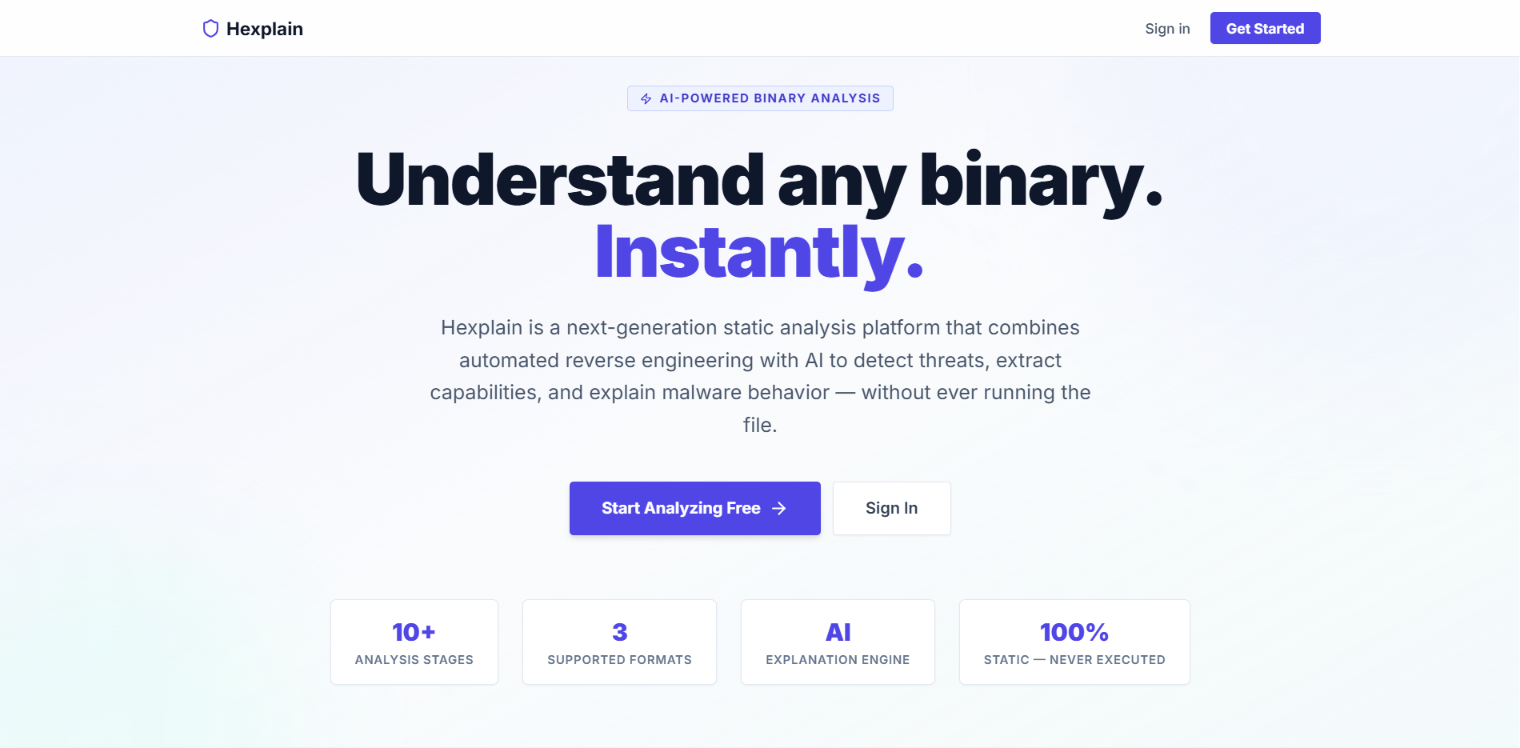
\includegraphics[width=\textwidth]{landing_page_hero}
  \caption{Page d'accueil de Hexplain --- \textit{«~Understand any binary. Instantly.~»}}
  \label{fig:landing_page}
\end{figure}

Le slogan --- \textit{«~Understand any binary. Instantly.~»} --- résume l'ambition fondamentale du projet~: démocratiser la compréhension des binaires en rendant l'analyse accessible en quelques secondes, sans expertise préalable en rétro-ingénierie.

\subsection{Authentification}

La page d'authentification propose une interface élégante avec deux onglets coulissants (Connexion / Inscription), illustrée en Figure~\ref{fig:auth_page}.

\begin{figure}[H]
  \centering
  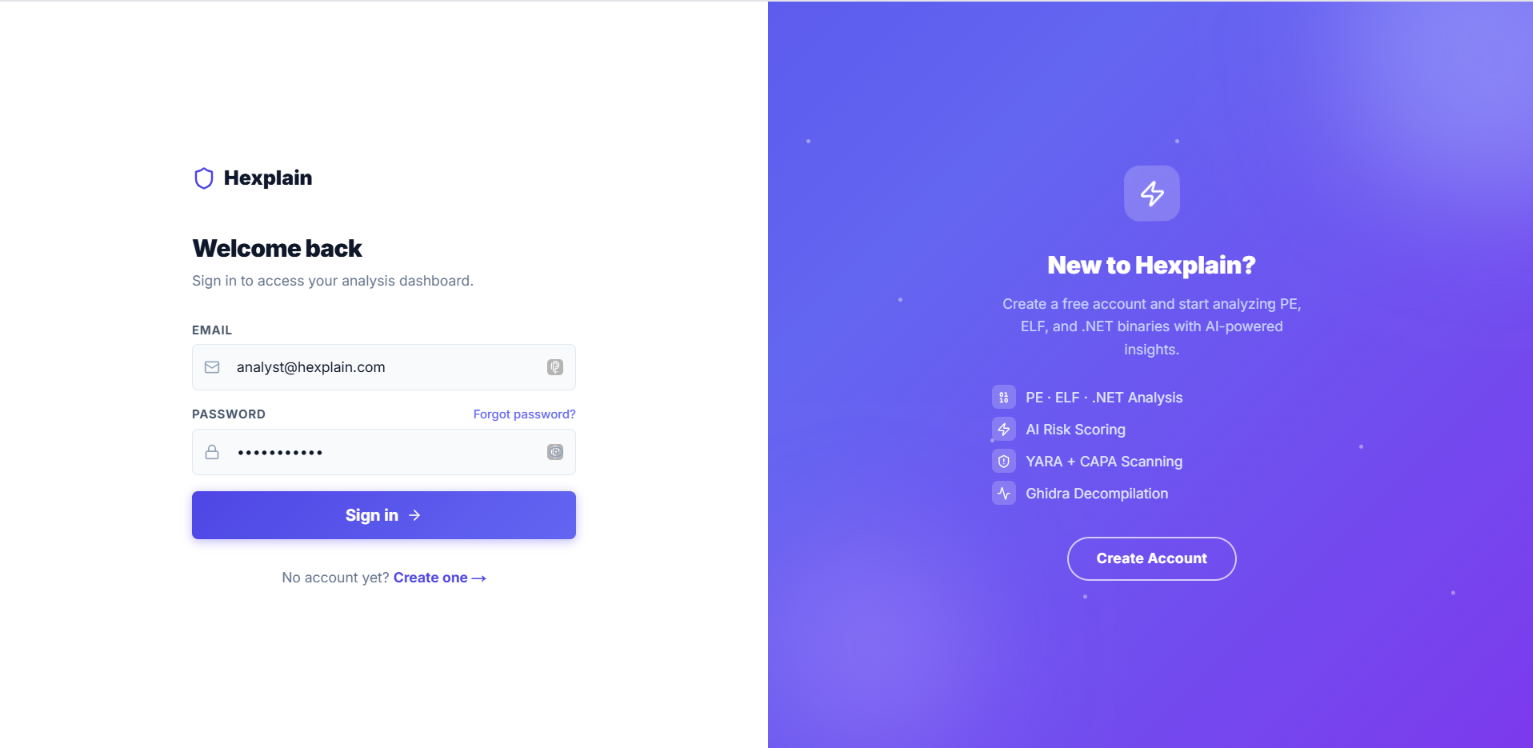
\includegraphics[width=\textwidth]{auth_login_page}
  \caption{Interface d'authentification --- vue onglet Connexion}
  \label{fig:auth_page}
\end{figure}

Techniquement, le formulaire de connexion~:
\begin{itemize}
  \item Envoie les identifiants via \texttt{POST /api/auth/login} avec le jeton CSRF dans l'en-tête \texttt{X-CSRF-Token}.
  \item Reçoit un cookie HttpOnly \texttt{access\_token} contenant le JWT signé.
  \item Redirige vers le tableau de bord en cas de succès, ou affiche un message d'erreur générique (sans préciser si c'est l'email ou le mot de passe qui est incorrect, pour ne pas aider un attaquant).
\end{itemize}

\subsection{Upload et soumission d'un binaire}

L'interface d'upload, présentée en Figure~\ref{fig:upload_interface}, permet à l'utilisateur de déposer un fichier (par glisser-déposer ou sélection) tout en affichant clairement les formats acceptés et les limites de taille.

\begin{figure}[H]
  \centering
  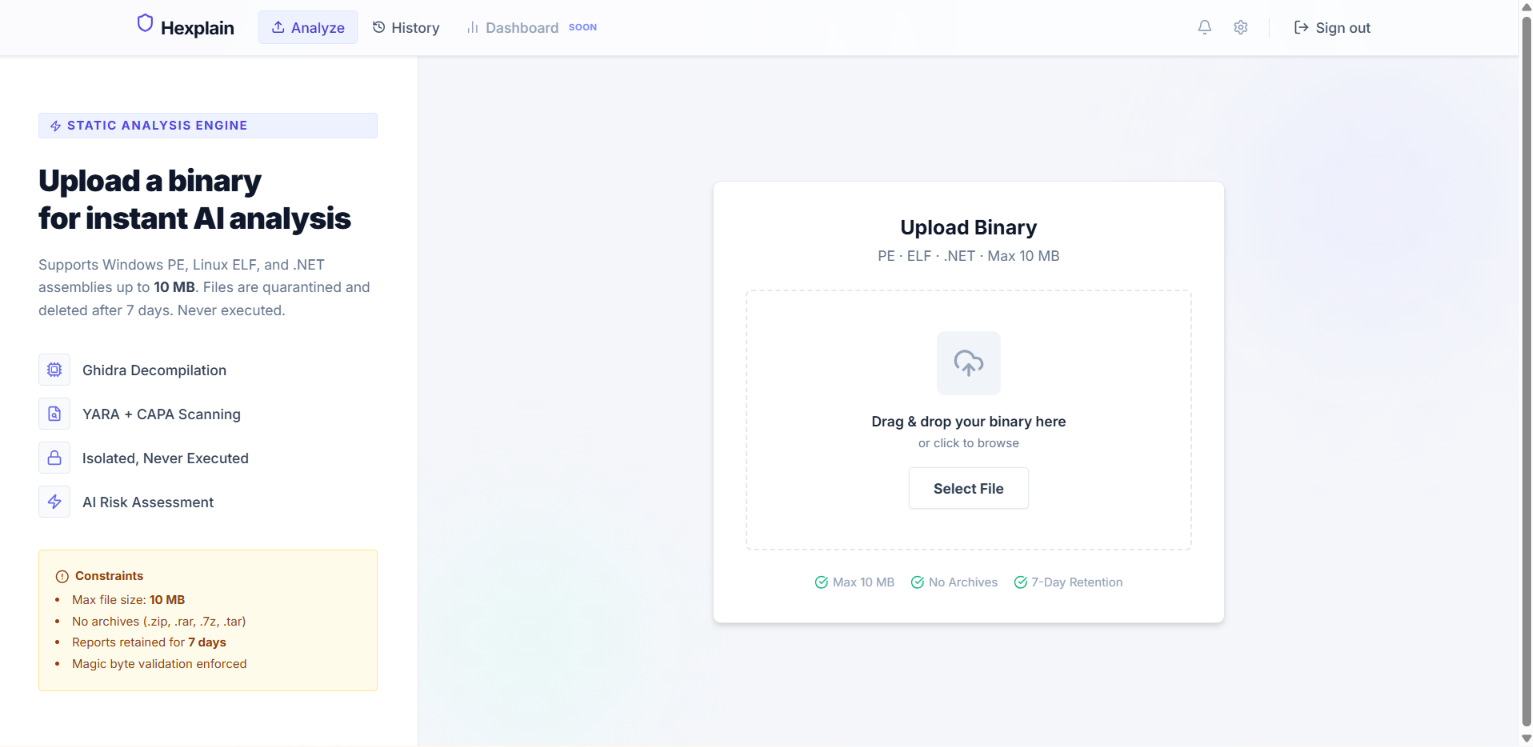
\includegraphics[width=\textwidth]{upload_binary_interface}
  \caption{Interface d'upload de binaires avec affichage des contraintes}
  \label{fig:upload_interface}
\end{figure}

Une fois le fichier soumis, l'API retourne immédiatement un \texttt{202 Accepted} avec le \texttt{job\_id}, et l'utilisateur est redirigé vers la page de suivi en temps réel.

\subsection{Suivi en temps réel du pipeline}

La page de suivi (Figure~\ref{fig:pipeline_progress}) affiche l'avancement de l'analyse en temps réel grâce à un mécanisme de \textit{polling} (interrogation périodique de l'API toutes les 3 secondes). Chaque module du pipeline est représenté par un indicateur d'état (en attente, en cours, terminé, en erreur).

\begin{figure}[H]
  \centering
  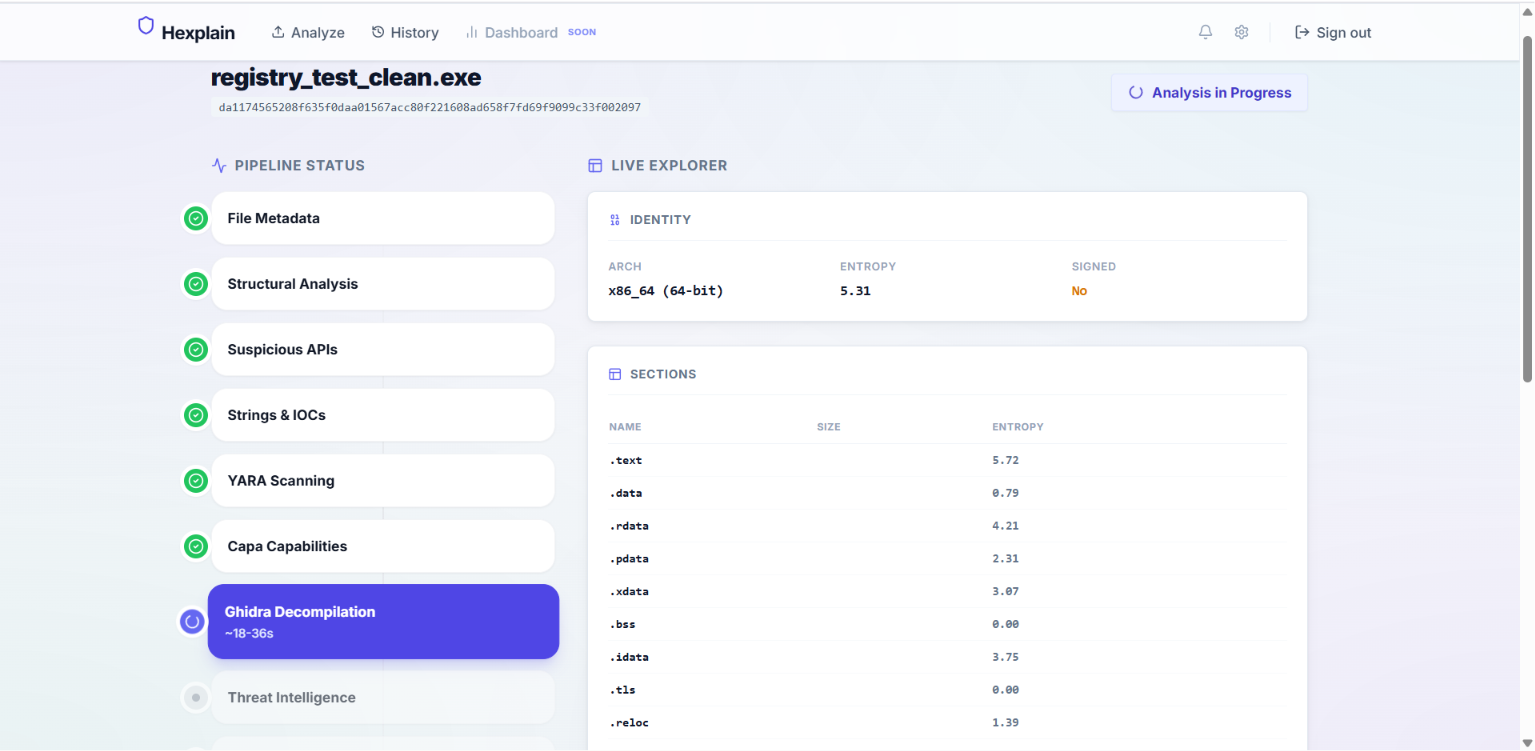
\includegraphics[width=\textwidth]{pipeline_live_progress}
  \caption{Écran de suivi en temps réel du pipeline d'analyse}
  \label{fig:pipeline_progress}
\end{figure}

La partie droite de l'écran propose un \textit{Live Explorer} qui donne accès aux résultats partiels des modules terminés, avant même la fin de l'analyse complète. Cette fonctionnalité améliore significativement l'expérience utilisateur en réduisant la perception du temps d'attente.

\subsection{Historique des analyses}

La page d'historique (Figure~\ref{fig:jobs_history}) liste toutes les analyses passées de l'utilisateur authentifié, avec leur nom de fichier, date, statut et score de risque affiché avec un badge coloré.

\begin{figure}[H]
  \centering
  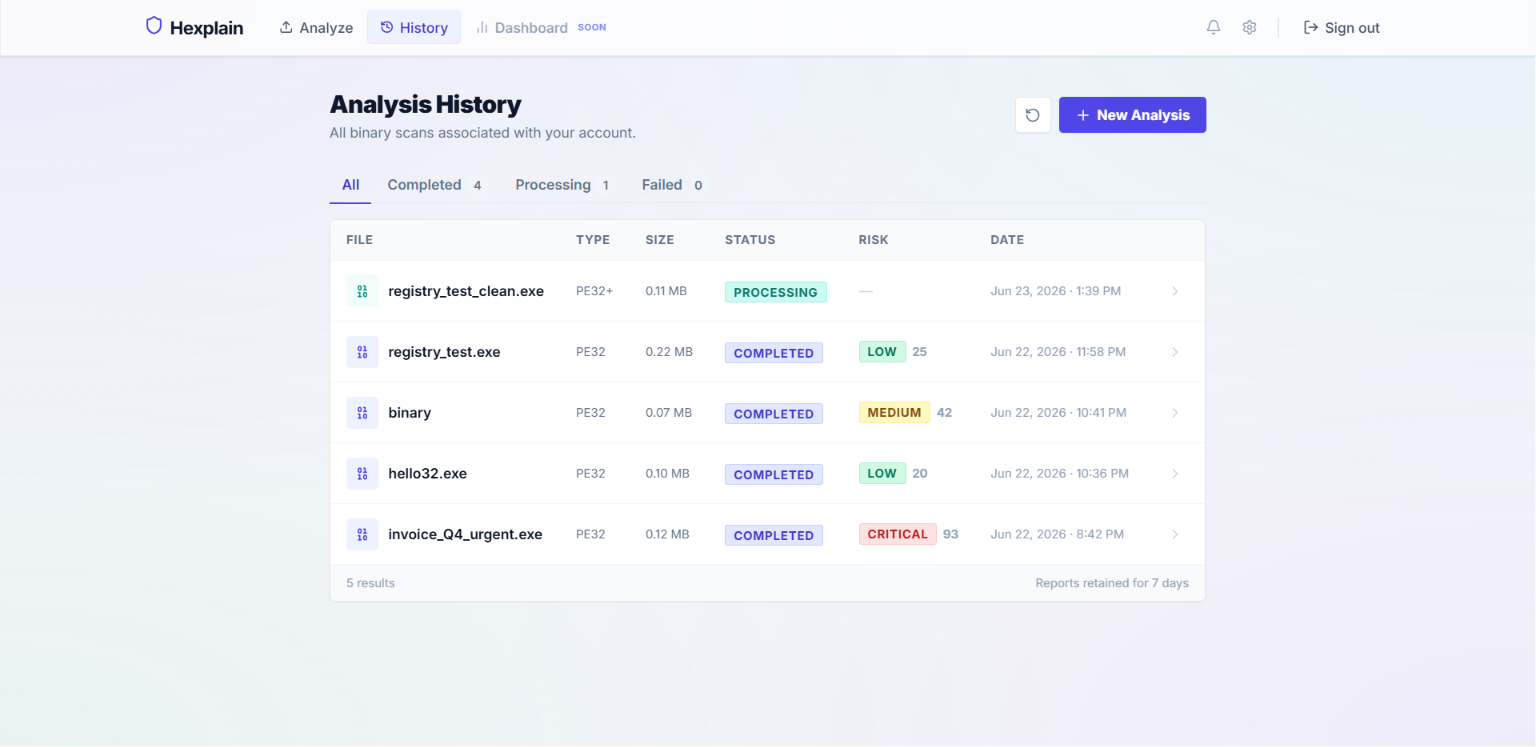
\includegraphics[width=0.9\textwidth]{jobs_history_list}
  \caption{Tableau de bord «~Analysis History~» avec scores de risque}
  \label{fig:jobs_history}
\end{figure}

\subsection{Rapport d'analyse complet}

Le rapport d'analyse est la fonctionnalité centrale de Hexplain. La Figure~\ref{fig:report_executive} montre la section de résumé exécutif, générée par le LLM~: classification, score de risque global, comportements clés détectés et correspondances YARA.

\begin{figure}[H]
  \centering
  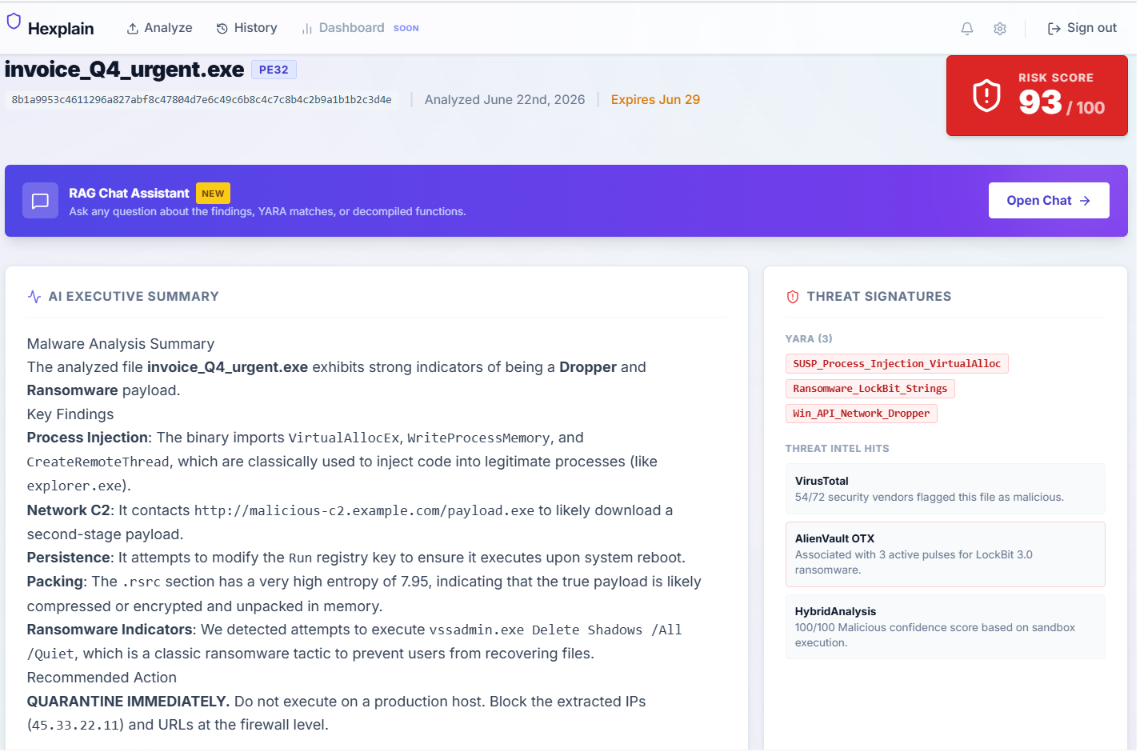
\includegraphics[width=\textwidth]{report_executive_summary}
  \caption{Rapport d'analyse --- résumé exécutif généré par LLM (score CRITICAL 93/100)}
  \label{fig:report_executive}
\end{figure}

La Figure~\ref{fig:report_capa} montre les sections dédiées aux capacités Capa, aux IOC extraits et à l'analyse des sections binaires avec leurs entropies. La section \texttt{.rsrc} est marquée «~PACKED?~» car son entropie (7.95) dépasse le seuil de 7.0.

\begin{figure}[H]
  \centering
  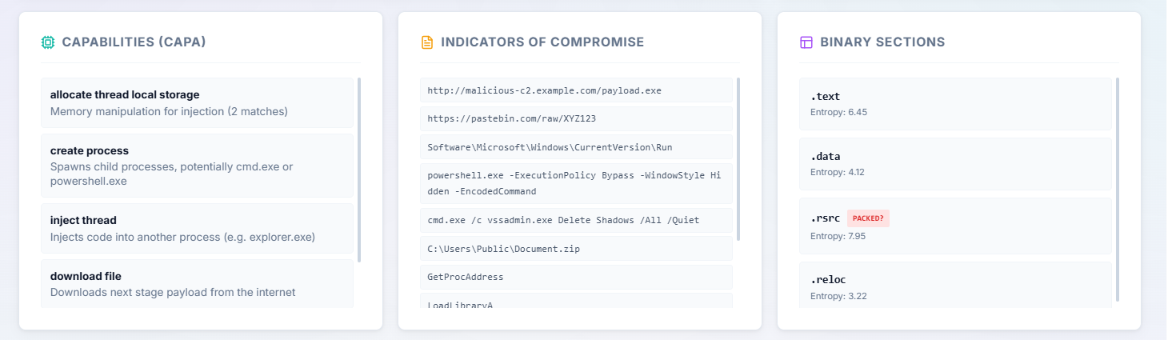
\includegraphics[width=\textwidth]{report_capa_iocs_sections}
  \caption{Rapport --- Capacités Capa, IOC détectés et analyse des sections binaires}
  \label{fig:report_capa}
\end{figure}

La Figure~\ref{fig:report_risk_breakdown} présente la décomposition du score de risque par facteur et la liste des fonctions décompilées par Ghidra avec leur nombre d'instructions.

\begin{figure}[H]
  \centering
  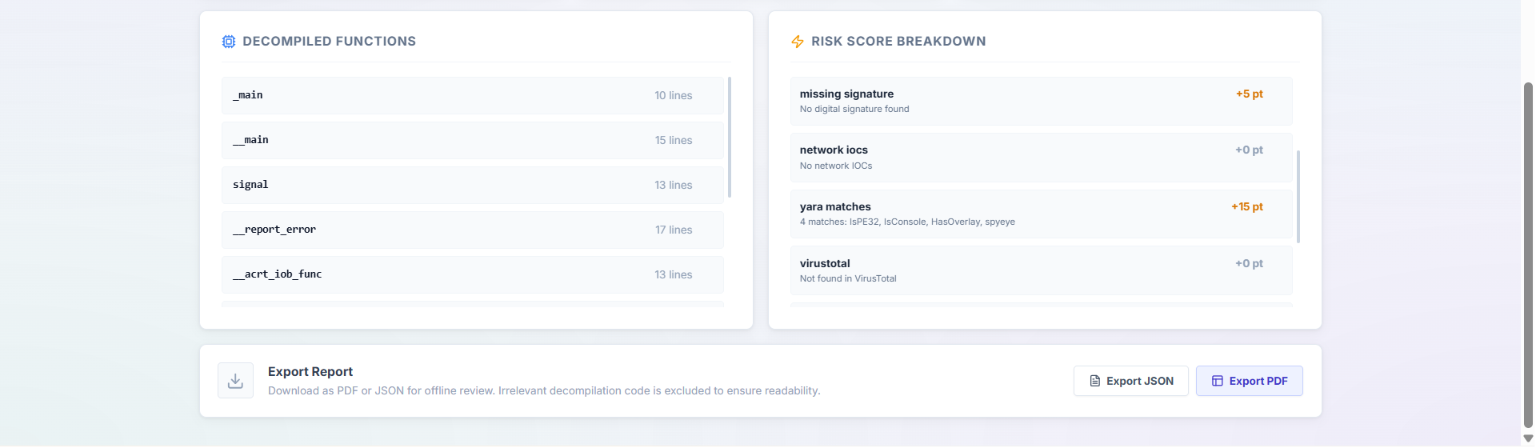
\includegraphics[width=\textwidth]{report_decompiled_functions_risk}
  \caption{Rapport --- Fonctions décompilées et détail du score de risque par facteur}
  \label{fig:report_risk_breakdown}
\end{figure}

\subsection{Vue décompilation --- Disassembleur et pseudo-C}

En cliquant sur une fonction dans le rapport, l'utilisateur accède à une vue dédiée (Figure~\ref{fig:disassembly_view}) présentant côte à côte le code assembleur brut (avec adresses mémoire et opcodes) et le pseudo-C généré par Ghidra, accompagné du bouton «~Explain Function~» pour obtenir une explication IA.

\begin{figure}[H]
  \centering
  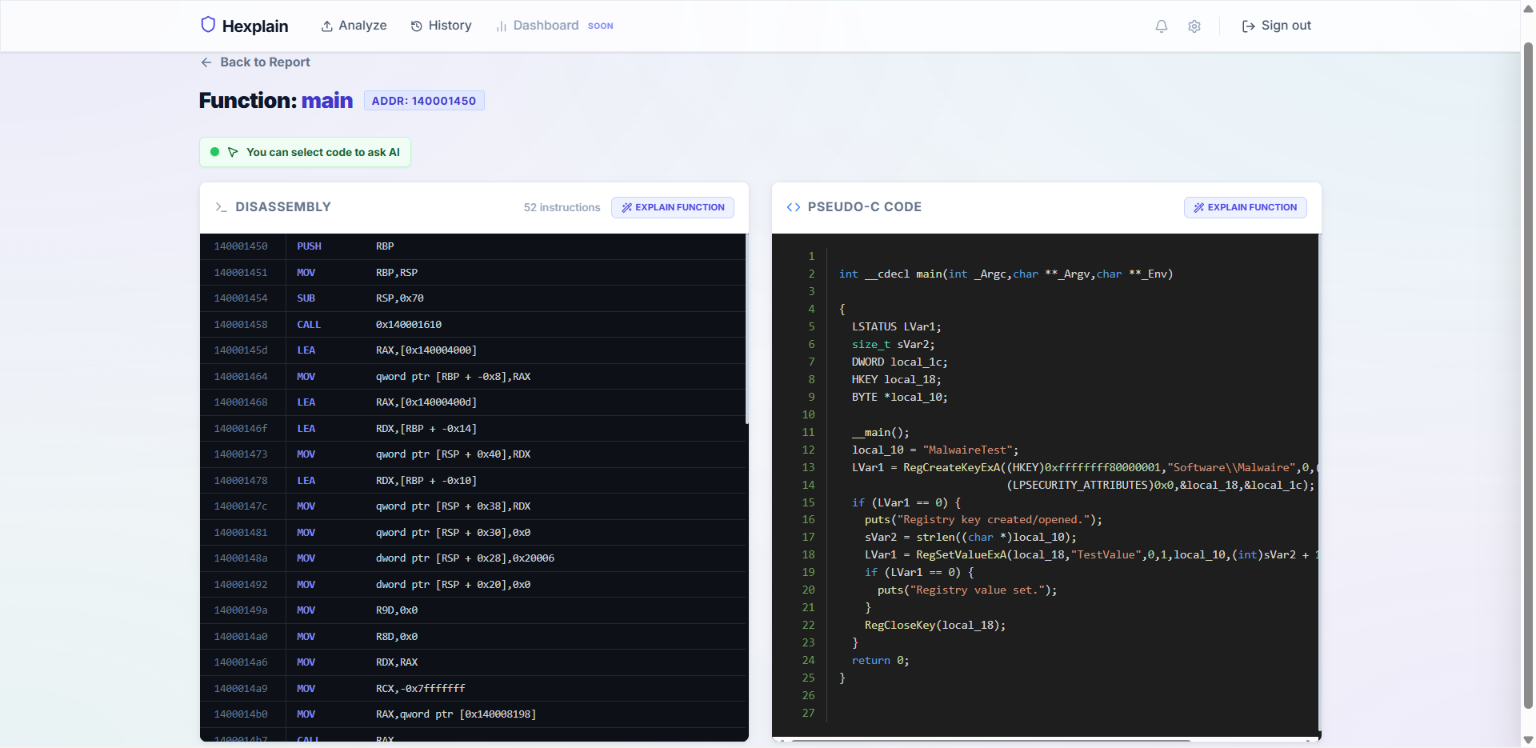
\includegraphics[width=\textwidth]{function_disassembly_pseudocode}
  \caption{Vue décompilation~: assembleur x86 (gauche) et pseudo-C Ghidra (droite)}
  \label{fig:disassembly_view}
\end{figure}

\subsection{Explication contextuelle par IA}

Le bouton «~Explain Function~» déclenche un appel LLM contextuel qui génère une explication pédagogique de la fonction sélectionnée (Figure~\ref{fig:ai_explanation}). L'explication est affichée dans un panneau latéral (\textit{drawer}), sans quitter la vue de décompilation.

\begin{figure}[H]
  \centering
  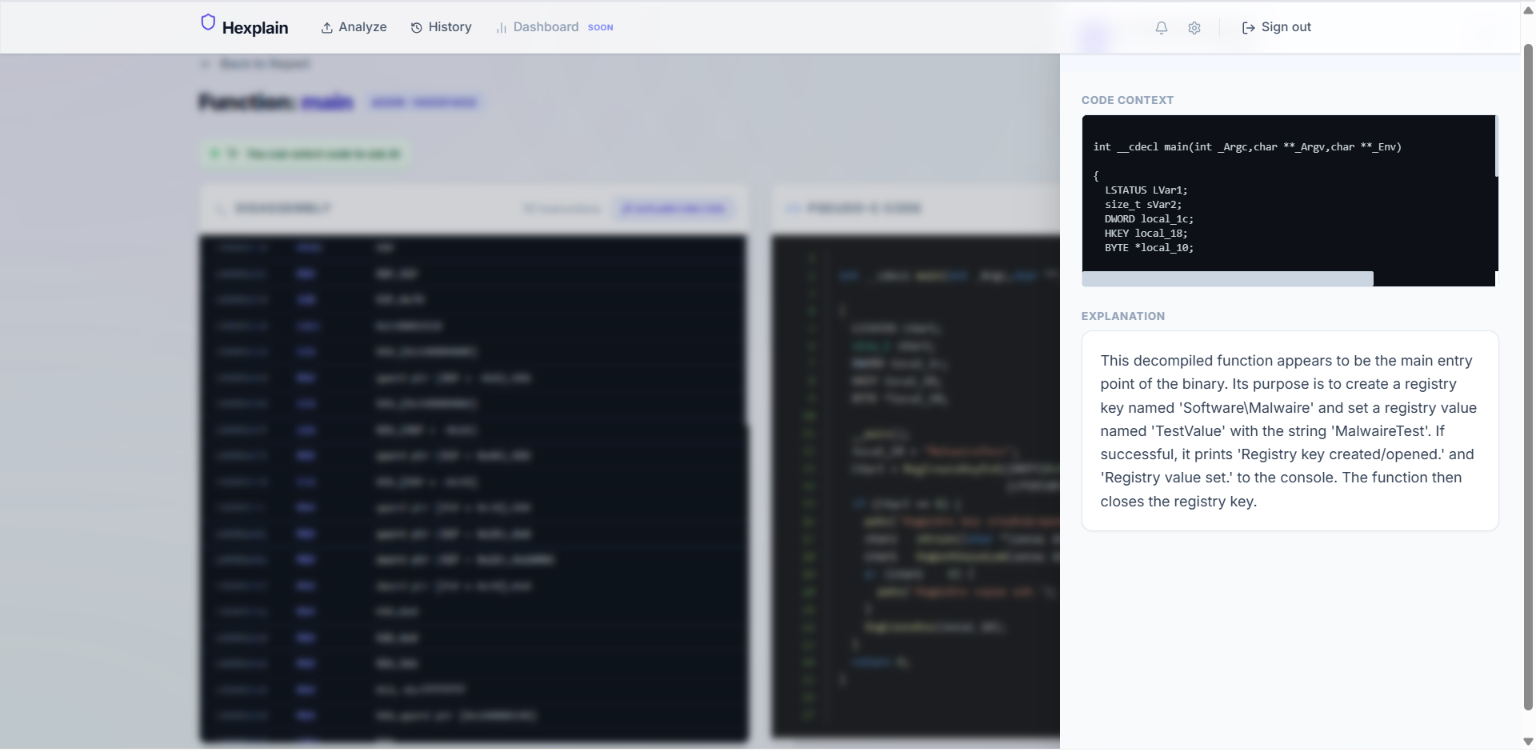
\includegraphics[width=\textwidth]{function_ai_explanation_drawer}
  \caption{Panneau d'explication IA contextuelle --- \textit{«~Explain Function~»}}
  \label{fig:ai_explanation}
\end{figure}

Ce mécanisme est également disponible pour les sections binaires (Figure~\ref{fig:section_ai_drawer})~: un bouton «~Ask AI About Section~» génère une explication contextuelle de la section sélectionnée (entropie, flags, implications de sécurité).

\begin{figure}[H]
  \centering
  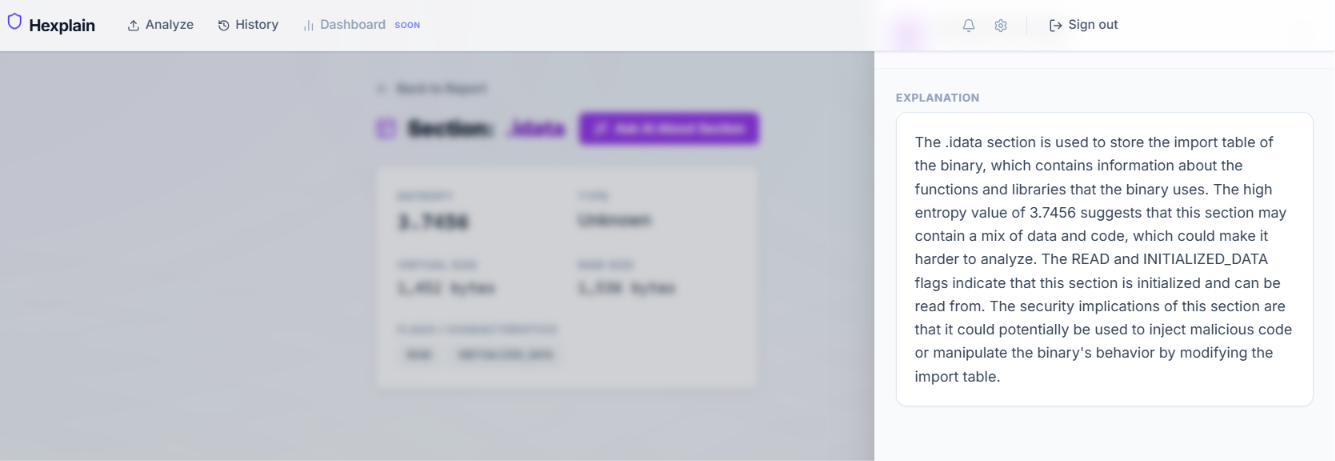
\includegraphics[width=0.9\textwidth]{section_detail_ai_drawer}
  \caption{Explication IA contextuelle d'une section binaire (.idata)}
  \label{fig:section_ai_drawer}
\end{figure}

\subsection{Détail d'une section binaire}

La page de détail d'une section (Figure~\ref{fig:section_idata}) présente ses caractéristiques techniques~: entropie de Shannon, type, taille virtuelle, taille brute et flags de caractéristiques (READ, WRITE, EXECUTE, INITIALIZED\_DATA).

\begin{figure}[H]
  \centering
  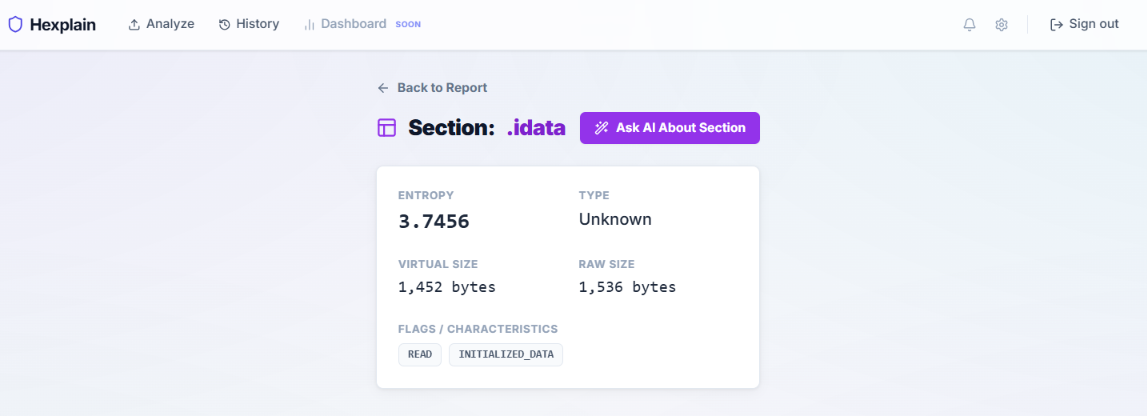
\includegraphics[width=0.7\textwidth]{section_idata_detail}
  \caption{Fiche détail de la section \texttt{.idata} (table des imports)}
  \label{fig:section_idata}
\end{figure}

\section{Chatbot RAG --- Copilote IA pédagogique}

\subsection{Interface du chatbot}

L'interface de chat IA (Figure~\ref{fig:rag_chat1}) permet à l'utilisateur de poser des questions en langage naturel sur l'analyse effectuée. Le chatbot répond en s'appuyant exclusivement sur le contenu indexé dans ChromaDB lors de la génération du rapport.

\begin{figure}[H]
  \centering
  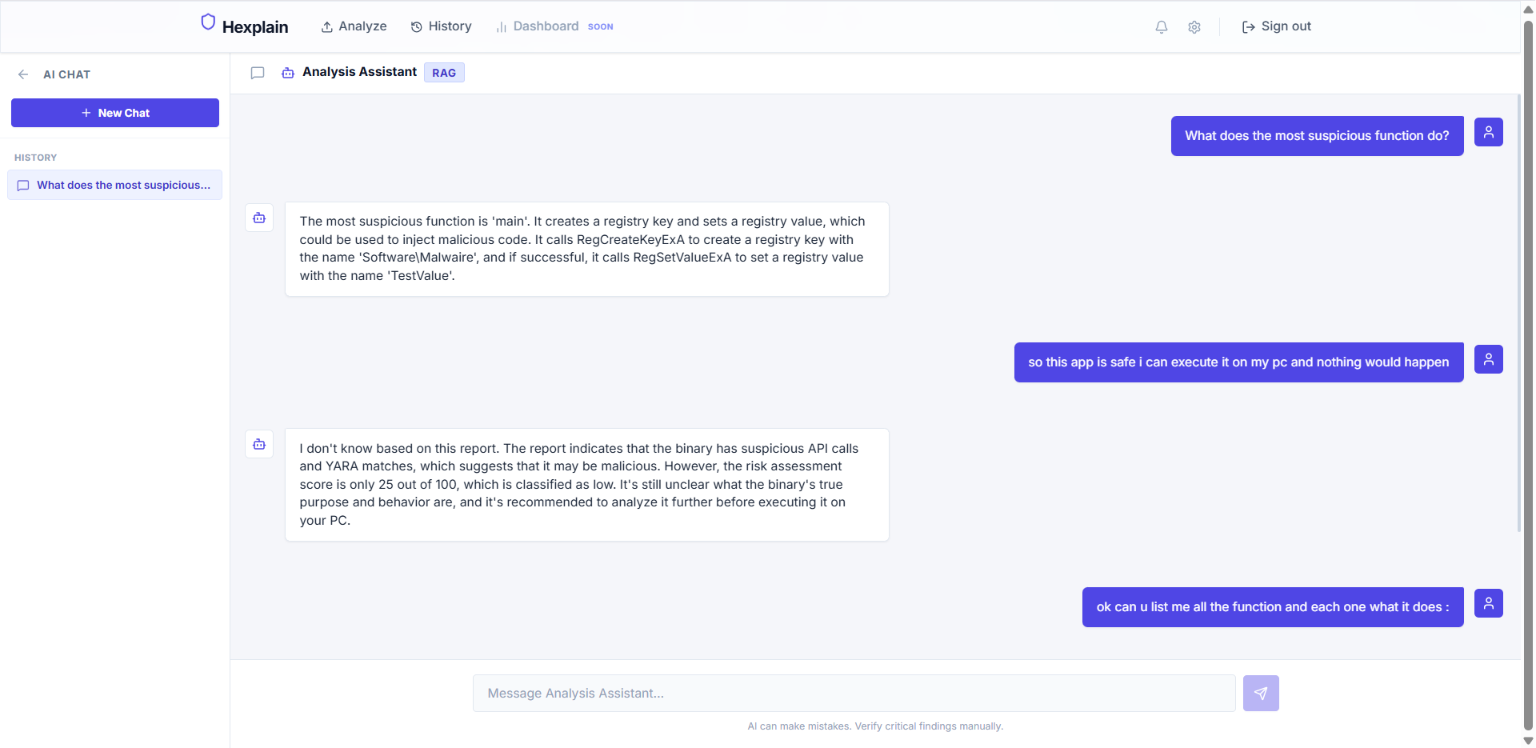
\includegraphics[width=\textwidth]{rag_chat_session1}
  \caption{Interface du chatbot RAG --- interrogation sur la fonction suspecte la plus critique}
  \label{fig:rag_chat1}
\end{figure}

\begin{figure}[H]
  \centering
  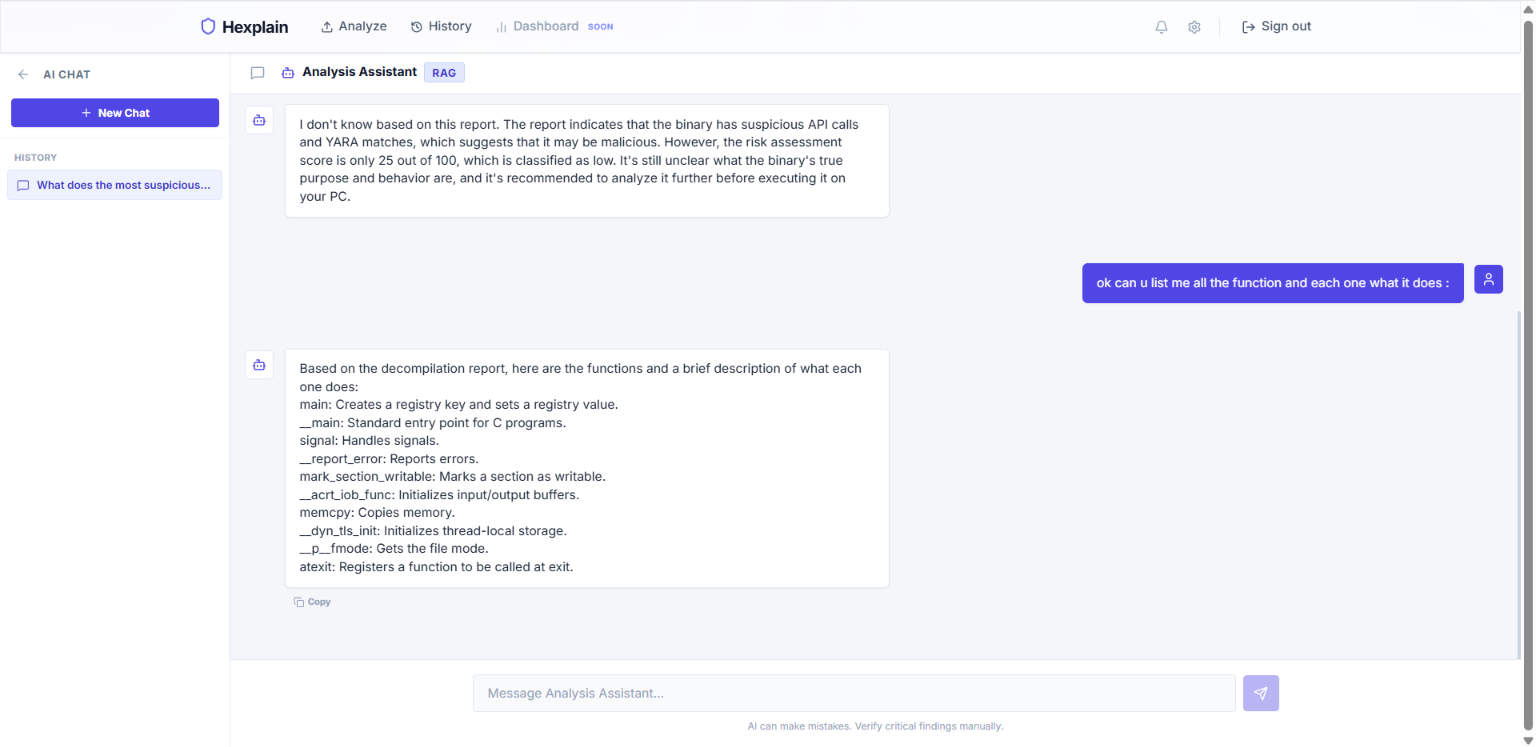
\includegraphics[width=\textwidth]{rag_chat_session2}
  \caption{Interface du chatbot RAG --- liste des fonctions décompilées avec rôles}
  \label{fig:rag_chat2}
\end{figure}

\subsection{Guardrails et prévention des hallucinations}

Plusieurs mécanismes ont été implémentés pour garantir la fiabilité des réponses du chatbot~:

\begin{itemize}
  \item \textbf{Anchoring explicite}~: Le prompt système instruit le LLM~: \textit{«~You must ONLY use the provided context to answer. If the answer is not in the context, say exactly: "I don't know based on this report."~»}
  \item \textbf{Injection de contexte limité}~: Seuls 5 chunks sémantiquement proches sont fournis au LLM, limitant la «~surface d'hallucination~» possible.
  \item \textbf{Contexte d'analyse obligatoire}~: Le LLM reçoit systématiquement en début de prompt le résumé général de l'analyse (type de fichier, score de risque, classification), lui évitant de devoir l'inférer.
  \item \textbf{Règle de sécurité stricte}~: Le LLM est explicitement instruit de ne jamais fournir d'instructions permettant de reproduire ou d'améliorer les techniques malveillantes identifiées dans le binaire.
\end{itemize}

\section{Export du rapport}

La plateforme propose deux formats d'export du rapport~:

\begin{itemize}
  \item \textbf{Export PDF}~: Généré côté client via \texttt{@react-pdf/renderer}, le rapport PDF (Figure~\ref{fig:pdf_export}) inclut le résumé exécutif, le score de risque, la liste des comportements clés, les correspondances YARA et les fonctions décompilées pertinentes.
  \item \textbf{Export JSON}~: Exporte le blob JSON complet du rapport (\texttt{report\_data}), permettant une intégration dans des outils SIEM ou des scripts d'automatisation.
\end{itemize}

\begin{figure}[H]
  \centering
  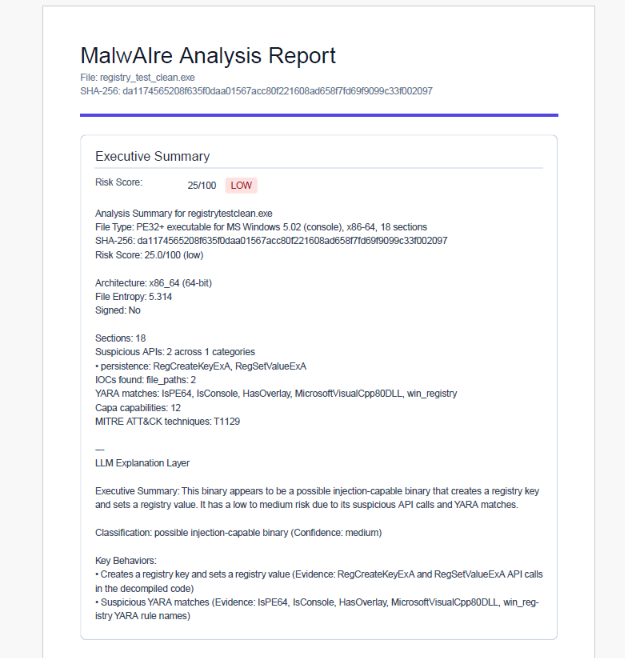
\includegraphics[width=0.65\textwidth]{pdf_export_report}
  \caption{Export PDF du rapport d'analyse MalwAIre (MalwAIre Analysis Report)}
  \label{fig:pdf_export}
\end{figure}

\section{Tests et validation}

\subsection{Tests du pipeline sur des binaires de référence}

Des tests ont été réalisés sur plusieurs binaires de démonstration~:

\begin{table}[H]
  \centering
  \caption{Résultats des tests sur binaires de démonstration}
  \label{tab:test_results}
  \begin{tabularx}{\textwidth}{l l c l X}
    \toprule
    \textbf{Fichier} & \textbf{Type} & \textbf{Score} & \textbf{Niveau} & \textbf{Détections clés} \\
    \midrule
    \texttt{registry\_test\_clean.exe} & PE32+ x64 & 25/100 & LOW & IsPE64, persistance registre, YARA \\
    \texttt{malware\_demo.exe} & PE32 x86 & 93/100 & CRITICAL & Injection (T1055), C2 URLs, 54/72 VT \\
    \texttt{sample\_elf} & ELF 64-bit & 42/100 & MEDIUM & Socket réseau, setuid, API chiffrement \\
    \bottomrule
  \end{tabularx}
\end{table}

\subsubsection{Analyse du binaire \texttt{registry\_test\_clean.exe}}

Ce binaire de démonstration (PE32+, x86-64, 18 sections, Score 25/100) a permis de valider le pipeline complet. Le LLM l'a correctement classifié comme «~possible injection-capable binary~» avec une confiance moyenne, identifiant les API \texttt{RegCreateKeyExA} et \texttt{RegSetValueExA} comme preuves d'une tentative de persistance via la clé \texttt{Software\textbackslash Malware} du registre Windows. Le score bas (25/100) est cohérent avec l'absence de détections VirusTotal et la simple persistance registre sans autres indicateurs de compromission.

\subsubsection{Validation du chatbot RAG}

Lors des tests de validation, le chatbot RAG a démontré sa capacité à~:
\begin{itemize}
  \item Répondre correctement aux questions factuelles («~Quel est le score de risque~?~», «~Quelles API suspectes ont été détectées~?~»).
  \item Décrire le rôle de chaque fonction décompilée en s'appuyant sur le contexte.
  \item Refuser explicitement de répondre aux questions hors contexte (ex.~: «~Comment puis-je utiliser cette technique~?~»).
  \item Gérer correctement la persistance de l'historique de conversation entre questions consécutives.
\end{itemize}

\subsection{Tests de sécurité}

\begin{itemize}
  \item \textbf{Test d'upload de fichier invalide}~: Un fichier PDF renommé \texttt{.exe} est rejeté avec une erreur 400 avant d'atteindre le système de fichiers (validation magic bytes en mémoire).
  \item \textbf{Test CSRF}~: Une requête POST sans en-tête \texttt{X-CSRF-Token} reçoit une réponse 403 Forbidden.
  \item \textbf{Test d'isolation inter-utilisateurs}~: Une requête \texttt{GET /api/jobs/{id}} avec un \texttt{job\_id} appartenant à un autre utilisateur reçoit une réponse 404 Not Found (pas de fuite d'existence du job).
  \item \textbf{Test de rate limiting}~: 6 tentatives de connexion en moins d'une minute depuis la même IP reçoivent une réponse 429 Too Many Requests.
\end{itemize}

\section{Conclusion}

Ce chapitre a documenté la réalisation complète de Hexplain, de l'interface utilisateur aux tests de validation. Les captures d'écran intégrées illustrent la cohérence et la richesse des fonctionnalités développées, couvrant l'intégralité du parcours utilisateur~: de l'upload du binaire au dialogue en langage naturel avec le copilote IA, en passant par la décompilation interactive et l'export du rapport. Les tests effectués ont confirmé la robustesse du pipeline d'analyse, l'efficacité des mécanismes de sécurité et la pertinence des réponses du chatbot RAG. Le chapitre suivant dresse le bilan du stage et expose les perspectives d'évolution du projet.

% =============================================================================
% Chapitre 6 — Bilan, limitations et perspectives
% =============================================================================

\chapter{Bilan, limitations et perspectives}

\section{Introduction}

Ce dernier chapitre avant la conclusion générale dresse un bilan objectif du projet Hexplain~: ce qui a été accompli, les limitations identifiées, et les pistes d'amélioration et d'évolution qui constitueront les prochaines étapes naturelles du projet. Il revient également sur les apports personnels et professionnels de ce stage.

\section{Bilan du projet}

\subsection{Objectifs atteints}

À l'issue des huit semaines de stage, l'ensemble des objectifs définis initialement ont été atteints~:

\begin{itemize}
  \item[\checkmark] \textbf{Pipeline d'analyse complet}~: Les 9 modules d'analyse statique sont opérationnels et intégrés dans un pipeline résilient géré par Celery.
  \item[\checkmark] \textbf{Couche LLM explicative}~: La génération de rapports en langage naturel fonctionne avec deux fournisseurs LLM (Gemini 2.0 Flash et Groq/Llama-3.1) avec basculement automatique.
  \item[\checkmark] \textbf{Chatbot RAG local}~: Le pipeline RAG (ChromaDB + sentence-transformers) est opérationnel avec des guardrails anti-hallucination validés.
  \item[\checkmark] \textbf{Interface web complète}~: Le dashboard Next.js 14 couvre l'intégralité du parcours utilisateur (upload, suivi, rapport, décompilation, chat, export).
  \item[\checkmark] \textbf{Sécurité}~: Les mécanismes de sécurité critiques (quarantaine, Argon2id, CSRF, rate limiting, isolation) sont tous opérationnels.
  \item[\checkmark] \textbf{Déploiement}~: La plateforme est déployée sur DigitalOcean avec CI/CD GitHub Actions.
\end{itemize}

\subsection{Métriques de développement}

Le projet représente un volume de code significatif~: \placeholder{Nombre de lignes de code exactes (à compter via \texttt{cloc} sur le dépôt)}. Les principales métriques disponibles sont~:

\begin{itemize}
  \item \textbf{Backend Python (FastAPI + Celery)}~: 9 modules d'analyse, 5 services transversaux (auth, LLM, RAG, threat intel, enrichissement IA).
  \item \textbf{Frontend TypeScript (Next.js)}~: Plus de 15 pages et composants couvrant l'ensemble du parcours utilisateur.
  \item \textbf{Docker}~: 4 conteneurs, 2 volumes persistants, 1 réseau interne.
  \item \textbf{Pipeline CI/CD}~: Déploiement automatisé en moins de 2 minutes sur push sur la branche \texttt{main}.
\end{itemize}

\section{Limitations du projet}

Un bilan objectif implique de reconnaître les limitations actuelles du système, qu'elles soient techniques, fonctionnelles ou liées aux contraintes du stage.

\subsection{Limitations techniques}

\subsubsection{Scalabilité limitée}
La contrainte \texttt{--concurrency=1} du Worker Celery, imposée par les besoins en RAM de Ghidra, signifie que la plateforme ne peut traiter qu'une analyse à la fois. En cas de fort trafic, les jobs s'accumulent dans la file d'attente et les utilisateurs peuvent attendre plusieurs minutes avant que leur analyse ne commence. Une architecture multi-workers avec des machines dédiées à Ghidra (et des workers légers pour les autres modules) serait nécessaire pour passer à l'échelle.

\subsubsection{Analyse statique uniquement}
Hexplain est, par conception, un outil d'analyse \textbf{statique} uniquement. Il ne collecte aucune information comportementale dynamique (appels système effectifs, modifications du registre observées à l'exécution, connexions réseau réelles). Pour les malwares fortement obfusqués, packés ou polymorphes, l'analyse statique seule peut manquer des comportements qui ne se révèlent qu'à l'exécution dans un environnement sandbox. La combinaison avec un outil d'analyse dynamique (Cuckoo Sandbox, CAPE) constitue une lacune à combler.

\subsubsection{Couverture de décompilation limitée pour les binaires obfusqués}
Ghidra peut échouer ou produire des pseudo-C peu lisibles face à des binaires fortement obfusqués (control flow obfuscation, bogus code, dead code injection). Le timeout de 120 secondes peut également être insuffisant pour des binaires très volumineux.

\subsubsection{Base de données SQLite}
SQLite est un excellent choix pour le développement et les usages mono-utilisateur, mais atteint ses limites en cas d'accès concurrents importants (plusieurs utilisateurs effectuant des analyses simultanément). La migration vers PostgreSQL est prévue mais non encore réalisée.

\subsubsection{Dépendance aux APIs externes}
Les modules de threat intelligence (VirusTotal, MalwareBazaar, OTX) et le module LLM (Groq/Gemini) dépendent de services externes avec des quotas d'utilisation. Le mode dégradé (sans LLM) a été prévu, mais une interruption de VirusTotal ou OTX dégrade la qualité du scoring heuristique.

\subsubsection{Pas d'analyse ARM / MIPS}
Ghidra supporte l'architecture ARM, mais les règles YARA, Capa et la liste d'API suspectes ont été optimisées pour x86/x64. L'analyse de binaires pour appareils embarqués (routeurs, IoT) est possible mais incomplète.

\subsection{Limitations fonctionnelles}

\subsubsection{Absence d'analyse des macros Office et des scripts}
Hexplain est conçu pour les binaires natifs PE/ELF/.NET. Il ne prend pas en charge l'analyse de macros Microsoft Office (\texttt{.docm}, \texttt{.xlsm}), de scripts PowerShell, de fichiers JavaScript malveillants ou de fichiers PDF. Ces formats représentent pourtant une part importante des vecteurs d'attaque modernes.

\subsubsection{Analyse réseau non implémentée}
Les adresses IP et URLs extraites des chaînes sont présentées comme IOC, mais Hexplain ne réalise pas de lookup de réputation d'IP/domaine en temps réel (sans appel à VirusTotal qui couvre déjà les hashes). Des services comme Shodan, IPInfo ou URLScan.io pourraient enrichir considérablement cette dimension.

\subsubsection{Absence de dashboard analytique}
Le Sprint 4 prévoyait un dashboard de visualisation analytique (distributions de scores, tendances temporelles, familles de malwares fréquentes). Cette fonctionnalité, marquée «~SOON~» dans la navigation, n'a pas été implémentée faute de temps.

\subsubsection{Pas de gestion des utilisateurs en rôle administrateur}
L'administration de la plateforme (gestion des utilisateurs, purge des analyses expirées, monitoring de la file Celery) doit être réalisée directement en base de données ou via l'interface Redis. Un panneau d'administration web n'a pas été développé.

\subsubsection{Règles YARA non personnalisables par l'utilisateur}
Les règles YARA sont fixées au déploiement. Un utilisateur avancé souhaitant ajouter ses propres règles doit accéder directement au système de fichiers du conteneur.

\section{Perspectives d'évolution}

Les limitations identifiées constituent autant de pistes de développement pour les versions futures de Hexplain.

\subsection{Perspectives techniques à court terme}

\begin{itemize}
  \item \textbf{Migration PostgreSQL}~: Remplacement de SQLite par PostgreSQL pour supporter la concurrence et les déploiements multi-instances.
  \item \textbf{Architecture multi-workers}~: Séparation du Worker en deux files~: une file «~légère~» pour les modules rapides (métadonnées, YARA, Capa) et une file «~lourde~» dédiée à Ghidra, permettant le traitement parallèle de plusieurs analyses.
  \item \textbf{Modèle d'embedding local plus performant}~: Remplacement de \textit{all-MiniLM-L6-v2} par un modèle spécialisé en cybersécurité (ex.~: \textit{SecBERT}~\cite{secbert2022}) pour améliorer la pertinence du retrieval RAG sur du vocabulaire technique spécialisé.
  \item \textbf{Cache des résultats par hash}~: Si un binaire avec le même SHA-256 a déjà été analysé, retourner directement le rapport cached sans relancer le pipeline. Réduction drastique du temps d'attente pour les fichiers fréquemment soumis.
\end{itemize}

\subsection{Perspectives fonctionnelles à moyen terme}

\begin{itemize}
  \item \textbf{Intégration d'un sandbox dynamique}~: Couplage avec Cuckoo Sandbox ou CAPE pour combiner analyse statique et dynamique dans un rapport unifié.
  \item \textbf{Support des macros Office et scripts}~: Extension du pipeline pour analyser les documents malveillants (\texttt{.docm}, \texttt{.xlsm}) via olevba/oletools, et les scripts PowerShell via des analyseurs statiques spécialisés.
  \item \textbf{Lookup de réputation IP/URL}~: Intégration de Shodan, URLScan.io ou IPInfo pour enrichir l'analyse des IOC réseau détectés dans les chaînes de caractères.
  \item \textbf{Dashboard analytique}~: Implémentation du tableau de bord avec visualisations D3.js~: distribution des scores de risque, familles de malwares détectées, évolution temporelle.
  \item \textbf{Upload par lots (batch)}~: Permettre à l'utilisateur de soumettre plusieurs binaires en une seule opération pour des analyses de campagne.
  \item \textbf{Règles YARA personnalisables}~: Interface d'édition et de test de règles YARA personnalisées directement depuis le dashboard.
  \item \textbf{Panneau d'administration}~: Interface de gestion des utilisateurs, monitoring de la file Celery et tableau de bord de santé de l'infrastructure.
\end{itemize}

\subsection{Perspectives à long terme}

\begin{itemize}
  \item \textbf{Modèle LLM spécialisé en sécurité}~: Fine-tuning d'un modèle de langage sur un corpus de rapports de malwares (Malware Analysis Reports, APT reports) pour améliorer la qualité et la précision des explications générées.
  \item \textbf{API publique / mode SaaS}~: Exposition d'une API publique documentée (OpenAPI) permettant l'intégration de Hexplain dans des pipelines SOC automatisés ou des outils tiers.
  \item \textbf{Plugin VirusTotal Community}~: Développement d'un plugin permettant de lancer une analyse Hexplain directement depuis la page VirusTotal d'un fichier.
  \item \textbf{Intégration MISP}~: Export automatique des IOC et des rapports au format MISP~\cite{misp2016} pour partage avec la communauté de threat intelligence.
  \item \textbf{Support multi-langues}~: Génération des rapports LLM en arabe, français, espagnol et anglais, pour rendre la plateforme accessible à un public international plus large.
\end{itemize}

\section{Apports personnels et professionnels}

Ce stage m'a permis d'acquérir et d'approfondir des compétences dans plusieurs domaines~:

\subsection{Compétences techniques acquises}
\begin{itemize}
  \item Maîtrise de l'analyse statique de binaires~: formats PE/ELF, entrée/sortie Ghidra, règles YARA, framework MITRE ATT\&CK.
  \item Conception et développement d'une API REST asynchrone avec FastAPI et Celery.
  \item Implémentation complète d'un pipeline RAG (Retrieval-Augmented Generation) avec ChromaDB et sentence-transformers.
  \item Ingénierie de prompts pour des LLM appliqués à la cybersécurité.
  \item Containerisation avancée avec Docker et Docker Compose (multi-services, volumes, healthchecks).
  \item Mise en place d'un pipeline CI/CD avec GitHub Actions.
  \item Développement frontend avec Next.js 14, TypeScript et Tailwind CSS.
  \item Application des principes de sécurité web~: Argon2id, JWT, CSRF, rate limiting, CSP.
\end{itemize}

\subsection{Compétences transverses développées}
\begin{itemize}
  \item Gestion de projet en mode agile (sprints de 2 semaines, réunions de suivi).
  \item Capacité à arbitrer entre ambition fonctionnelle et contraintes de temps.
  \item Rédaction de documentation technique en anglais.
  \item Communication régulière avec l'encadrant professionnel~: formulation claire des blocages, propositions de solutions alternatives.
  \item Travail en autonomie sur une problématique à la frontière de deux domaines (sécurité et IA).
\end{itemize}

\section{Conclusion}

Ce chapitre a dressé un bilan honnête et complet du projet Hexplain. Si l'ensemble des objectifs définis en début de stage ont été atteints, plusieurs limitations subsistent~: scalabilité du Worker, couverture des formats de fichiers, absence du dashboard analytique. Ces limitations ne sont pas des échecs mais des priorités identifiées pour les prochaines versions, qui bénéficient d'une feuille de route claire. Le stage a constitué une expérience formatrice exceptionnelle, permettant d'explorer à la fois les profondeurs de la rétro-ingénierie binaire et les possibilités offertes par les LLM appliqués à la cybersécurité, dans un environnement professionnel stimulant et bienveillant.

% =============================================================================
% Conclusion générale
% =============================================================================

\chapter*{Conclusion générale}
\addcontentsline{toc}{chapter}{Conclusion générale}
\markboth{Conclusion générale}{Conclusion générale}

Ce rapport de stage a présenté la conception, le développement et le déploiement de \textbf{Hexplain}, une plateforme d'analyse statique de binaires PE/ELF intégrant des modèles de langage de grande taille (LLM) pour la génération automatique de rapports de cybersécurité.

\section*{Synthèse des travaux réalisés}

Partant d'un constat simple mais fondamental --- la compréhension du code assembleur et des outils d'analyse statique constitue une barrière réelle à l'adoption de bonnes pratiques de cybersécurité --- nous avons conçu et développé une solution complète répondant à ce défi. Le pipeline Hexplain enchaîne neuf modules d'analyse automatisés~: extraction de métadonnées, analyse structurelle, détection d'API suspectes, extraction d'IOC, scan YARA, détection de capacités MITRE ATT\&CK via Capa, décompilation Ghidra/ILSpy, renseignements sur les menaces et scoring heuristique. Ces résultats, consolidés par un LLM (Gemini 2.0 Flash / Llama-3.1), donnent naissance à un rapport d'analyse pédagogique en langage naturel, accompagné d'un score de risque hybride (heuristique + IA) sur 100 points.

La couche RAG (\textit{Retrieval-Augmented Generation}), fondée sur ChromaDB et le modèle \textit{sentence-transformers} all-MiniLM-L6-v2, offre en complément un chatbot pédagogique permettant à l'utilisateur de dialoguer interactivement avec le rapport généré, en posant des questions en langage naturel sur les comportements détectés. Des guardrails stricts garantissent que les réponses sont exclusivement ancrées dans les données du rapport, sans fabrication d'informations.

Sur le plan de la sécurité --- préoccupation centrale quand on manipule des logiciels malveillants --- le système intègre des mécanismes robustes à chaque couche~: hachage Argon2id des mots de passe, JWT en cookies HttpOnly, protection CSRF par double-submit, isolation physique des binaires en quarantaine, validation en deux passes des fichiers, cloisonnement réseau Docker et limitation de débit des endpoints d'authentification. Aucun binaire analysé n'est jamais exécuté par la plateforme.

L'ensemble a été déployé avec succès sur une infrastructure DigitalOcean Droplet via Docker Compose, avec un pipeline CI/CD GitHub Actions garantissant des déploiements automatisés et fiables.

\section*{Valeur ajoutée et impact}

Hexplain se distingue des solutions existantes par l'originalité de son positionnement~: il ne remplace pas l'analyste expert, mais le démultiplie. Pour l'analyste débutant, il fournit une explication pédagogique des sorties brutes qu'il n'aurait pas su interpréter seul. Pour l'analyste expérimenté, il automatise les tâches répétitives (lookup VT, compilation YARA, extraction d'IOC) et génère une première ébauche de rapport qu'il peut valider et enrichir en quelques minutes au lieu de plusieurs heures.

Cette approche est particulièrement pertinente dans le contexte africain et des pays en développement, où les ressources humaines spécialisées en cybersécurité sont rares et les budgets pour les solutions commerciales souvent insuffisants. Hexplain démontre qu'une solution performante et sécurisée peut être déployée à faible coût, en s'appuyant sur des APIs gratuites et des outils open-source.

\section*{Apports du stage}

Ce stage a représenté une expérience formatrice à plusieurs niveaux. Sur le plan technique, il m'a permis d'acquérir une compréhension profonde de l'analyse statique de malwares --- un domaine que j'avais abordé en cours mais dont j'ai vraiment appréhendé la complexité au contact du code et des outils réels. Il m'a également permis de mettre en pratique l'ingénierie LLM dans un contexte professionnel concret, bien loin des tutoriels~: concevoir un prompt system rigoureux, gérer les guardrails, arbitrer entre qualité et coût d'inférence.

Sur le plan humain et professionnel, travailler au sein d'AIOX Labs m'a confronté à la réalité d'un environnement de startup innovante~: l'autonomie dans les choix techniques, la nécessité de justifier ses décisions d'architecture, la gestion des blocages (intégration Ghidra dans Docker), et la satisfaction de voir une idée prendre forme jusqu'au déploiement en production.

\section*{Perspectives}

Les perspectives identifiées dans le Chapitre 6 ouvrent des horizons prometteurs~: migration vers PostgreSQL, architecture multi-workers, intégration d'un sandbox dynamique, support des macros Office, fine-tuning d'un LLM spécialisé en cybersécurité. Ces évolutions constituent une feuille de route claire pour un projet qui pourrait, à terme, évoluer vers une offre SaaS à destination des équipes SOC et des organisations souhaitant renforcer leurs capacités d'analyse de menaces sans investissement massif en expertise humaine.

\vspace{1cm}

\noindent Hexplain est la démonstration concrète qu'en combinant judicieusement l'analyse statique éprouvée, la puissance des LLM et une architecture sécurisée rigoureuse, il est possible de démocratiser la compréhension des logiciels malveillants et de rendre la cybersécurité avancée accessible à un public bien plus large que le cercle restreint des experts en rétro-ingénierie.


% =========================================================
% BIBLIOGRAPHIE
% =========================================================
\printbibliography[heading=bibintoc, title={Références et Bibliographie}]

% =========================================================
% GLOSSAIRE & ACRONYMES
% =========================================================
\printglossary[type=\acronymtype, title={Liste des Sigles et Acronymes}, toctitle={Liste des Sigles et Acronymes}]

\end{document}
